\documentclass{book}
\usepackage[a4paper,top=2.5cm,bottom=2.5cm,left=2.5cm,right=2.5cm]{geometry}
\usepackage{makeidx}
\usepackage{natbib}
\usepackage{graphicx}
\usepackage{multicol}
\usepackage{float}
\usepackage{listings}
\usepackage{color}
\usepackage{ifthen}
\usepackage[table]{xcolor}
\usepackage{textcomp}
\usepackage{alltt}
\usepackage{ifpdf}
\ifpdf
\usepackage[pdftex,
            pagebackref=true,
            colorlinks=true,
            linkcolor=blue,
            unicode
           ]{hyperref}
\else
\usepackage[ps2pdf,
            pagebackref=true,
            colorlinks=true,
            linkcolor=blue,
            unicode
           ]{hyperref}
\usepackage{pspicture}
\fi
\usepackage[utf8]{inputenc}
\usepackage{mathptmx}
\usepackage[scaled=.90]{helvet}
\usepackage{courier}
\usepackage{sectsty}
\usepackage{amssymb}
\usepackage[titles]{tocloft}
\usepackage{doxygen}
\lstset{language=C++,inputencoding=utf8,basicstyle=\footnotesize,breaklines=true,breakatwhitespace=true,tabsize=4,numbers=left }
\makeindex
\setcounter{tocdepth}{3}
\renewcommand{\footrulewidth}{0.4pt}
\renewcommand{\familydefault}{\sfdefault}
\hfuzz=15pt
\setlength{\emergencystretch}{15pt}
\hbadness=750
\tolerance=750
\begin{document}
\hypersetup{pageanchor=false,citecolor=blue}
\begin{titlepage}
\vspace*{7cm}
\begin{center}
{\Large H\-A\-L }\\
\vspace*{1cm}
{\large Generated by Doxygen 1.8.3.1}\\
\vspace*{0.5cm}
{\small Mon Mar 31 2014 00:19:27}\\
\end{center}
\end{titlepage}
\clearemptydoublepage
\pagenumbering{roman}
\tableofcontents
\clearemptydoublepage
\pagenumbering{arabic}
\hypersetup{pageanchor=true,citecolor=blue}
\chapter{The H.\-E.\-P. Analysis Library}
\label{index}\hypertarget{index}{}\hypertarget{index_intro_sec}{}\section{Introduction}\label{index_intro_sec}
This a custom R\-O\-O\-T library that provides a framework for physics analysis. It contains several functions and classes that aid in analyzing high energy physics data. To aid in the compilation of all the source code, a macro entitled {\ttfamily Compile\-Source.\-C} can be executed from the command line. All functions and classes are available in python from the {\ttfamily lib/\-H\-A\-L.\-py} module. Furthermore, everything lives in the 'H\-A\-L' namespace. H\-A\-L stands for\par
 H -\/ H.\-E.\-P.\par
 A -\/ Analysis\par
 L -\/ Library\par
 Of course, this is also a thinly veiled reference to the villian in the classic \char`\"{}2001\-: A Space Odyssey.\char`\"{} But, I personally think this bit of software is far less pernicious 
\chapter{Hierarchical Index}
\section{Class Hierarchy}
This inheritance list is sorted roughly, but not completely, alphabetically\-:\begin{DoxyCompactList}
\item \contentsline{section}{H\-A\-L\-:\-:Algorithm}{\pageref{class_h_a_l_1_1_algorithm}}{}
\begin{DoxyCompactList}
\item \contentsline{section}{H\-A\-L\-:\-:Cut\-Algorithm}{\pageref{class_h_a_l_1_1_cut_algorithm}}{}
\item \contentsline{section}{H\-A\-L\-:\-:F\-A0000}{\pageref{class_h_a_l_1_1_f_a0000}}{}
\item \contentsline{section}{H\-A\-L\-:\-:Import\-T\-L\-V\-Algo}{\pageref{class_h_a_l_1_1_import_t_l_v_algo}}{}
\begin{DoxyCompactList}
\item \contentsline{section}{H\-A\-L\-:\-:I\-A0000}{\pageref{class_h_a_l_1_1_i_a0000}}{}
\item \contentsline{section}{H\-A\-L\-:\-:I\-A0001}{\pageref{class_h_a_l_1_1_i_a0001}}{}
\item \contentsline{section}{H\-A\-L\-:\-:I\-A0002}{\pageref{class_h_a_l_1_1_i_a0002}}{}
\item \contentsline{section}{H\-A\-L\-:\-:I\-A0010}{\pageref{class_h_a_l_1_1_i_a0010}}{}
\item \contentsline{section}{H\-A\-L\-:\-:I\-A0011}{\pageref{class_h_a_l_1_1_i_a0011}}{}
\item \contentsline{section}{H\-A\-L\-:\-:I\-A0012}{\pageref{class_h_a_l_1_1_i_a0012}}{}
\item \contentsline{section}{H\-A\-L\-:\-:I\-A0020}{\pageref{class_h_a_l_1_1_i_a0020}}{}
\item \contentsline{section}{H\-A\-L\-:\-:I\-A0021}{\pageref{class_h_a_l_1_1_i_a0021}}{}
\item \contentsline{section}{H\-A\-L\-:\-:I\-A0022}{\pageref{class_h_a_l_1_1_i_a0022}}{}
\end{DoxyCompactList}
\item \contentsline{section}{H\-A\-L\-:\-:Reconstruction\-Algorithm}{\pageref{class_h_a_l_1_1_reconstruction_algorithm}}{}
\begin{DoxyCompactList}
\item \contentsline{section}{H\-A\-L\-:\-:Python\-Reconstruction\-Algorithm}{\pageref{class_h_a_l_1_1_python_reconstruction_algorithm}}{}
\end{DoxyCompactList}
\end{DoxyCompactList}
\item \contentsline{section}{H\-A\-L\-:\-:Analysis}{\pageref{class_h_a_l_1_1_analysis}}{}
\item \contentsline{section}{H\-A\-L\-:\-:Cut\-Optimizer}{\pageref{class_h_a_l_1_1_cut_optimizer}}{}
\item exception\begin{DoxyCompactList}
\item \contentsline{section}{H\-A\-L\-:\-:H\-A\-L\-Exception}{\pageref{class_h_a_l_1_1_h_a_l_exception}}{}
\end{DoxyCompactList}
\item \contentsline{section}{H\-A\-L\-:\-:Integrator}{\pageref{class_h_a_l_1_1_integrator}}{}
\item \contentsline{section}{H\-A\-L\-:\-:Interp\-Base}{\pageref{class_h_a_l_1_1_interp_base}}{}
\begin{DoxyCompactList}
\item \contentsline{section}{H\-A\-L\-:\-:Poly\-Interp}{\pageref{class_h_a_l_1_1_poly_interp}}{}
\end{DoxyCompactList}
\item \contentsline{section}{H\-A\-L\-:\-:Poly2\-D\-Interp}{\pageref{class_h_a_l_1_1_poly2_d_interp}}{}
\item T\-Named\begin{DoxyCompactList}
\item \contentsline{section}{H\-A\-L\-:\-:Analysis\-Data}{\pageref{class_h_a_l_1_1_analysis_data}}{}
\begin{DoxyCompactList}
\item \contentsline{section}{H\-A\-L\-:\-:Analysis\-Tree\-Writer}{\pageref{class_h_a_l_1_1_analysis_tree_writer}}{}
\end{DoxyCompactList}
\item \contentsline{section}{H\-A\-L\-:\-:Analysis\-Tree\-Reader}{\pageref{class_h_a_l_1_1_analysis_tree_reader}}{}
\end{DoxyCompactList}
\item T\-Selector\begin{DoxyCompactList}
\item \contentsline{section}{H\-A\-L\-:\-:Analysis\-Selector}{\pageref{class_h_a_l_1_1_analysis_selector}}{}
\end{DoxyCompactList}
\end{DoxyCompactList}

\chapter{Class Index}
\section{Class List}
Here are the classes, structs, unions and interfaces with brief descriptions\+:\begin{DoxyCompactList}
\item\contentsline{section}{\hyperlink{class_h_a_l_1_1_algorithm}{H\+A\+L\+::\+Algorithm} }{\pageref{class_h_a_l_1_1_algorithm}}{}
\item\contentsline{section}{\hyperlink{class_h_a_l_1_1_analysis}{H\+A\+L\+::\+Analysis} }{\pageref{class_h_a_l_1_1_analysis}}{}
\item\contentsline{section}{\hyperlink{class_h_a_l_1_1_analysis_data}{H\+A\+L\+::\+Analysis\+Data} }{\pageref{class_h_a_l_1_1_analysis_data}}{}
\item\contentsline{section}{\hyperlink{class_h_a_l_1_1_analysis_selector}{H\+A\+L\+::\+Analysis\+Selector} }{\pageref{class_h_a_l_1_1_analysis_selector}}{}
\item\contentsline{section}{\hyperlink{class_h_a_l_1_1_analysis_tree_reader}{H\+A\+L\+::\+Analysis\+Tree\+Reader} }{\pageref{class_h_a_l_1_1_analysis_tree_reader}}{}
\item\contentsline{section}{\hyperlink{class_h_a_l_1_1_analysis_tree_writer}{H\+A\+L\+::\+Analysis\+Tree\+Writer} }{\pageref{class_h_a_l_1_1_analysis_tree_writer}}{}
\item\contentsline{section}{\hyperlink{class_h_a_l_1_1_algorithms_1_1_attach_attribute}{H\+A\+L\+::\+Algorithms\+::\+Attach\+Attribute} \\*\hyperlink{class_h_a_l_1_1_algorithm}{Algorithm} that attaches a decimal value to an existing set of particles }{\pageref{class_h_a_l_1_1_algorithms_1_1_attach_attribute}}{}
\item\contentsline{section}{\hyperlink{class_h_a_l_1_1_algorithms_1_1_cut}{H\+A\+L\+::\+Algorithms\+::\+Cut} \\*Generic algorithm class that cuts on particle multiplicity, bool, integer, counting, and decimal values }{\pageref{class_h_a_l_1_1_algorithms_1_1_cut}}{}
\item\contentsline{section}{\hyperlink{class_h_a_l_1_1_cut_algorithm}{H\+A\+L\+::\+Cut\+Algorithm} }{\pageref{class_h_a_l_1_1_cut_algorithm}}{}
\item\contentsline{section}{\hyperlink{class_h_a_l_1_1_cut_optimizer}{H\+A\+L\+::\+Cut\+Optimizer} }{\pageref{class_h_a_l_1_1_cut_optimizer}}{}
\item\contentsline{section}{\hyperlink{class_h_a_l_1_1_algorithms_1_1_empty_cut}{H\+A\+L\+::\+Algorithms\+::\+Empty\+Cut} \\*Generic algorithm class that serves as a baseline algorithm for any subsequent \hyperlink{class_h_a_l_1_1_algorithms_1_1_cut}{Cut} algorithms }{\pageref{class_h_a_l_1_1_algorithms_1_1_empty_cut}}{}
\item\contentsline{section}{\hyperlink{class_h_a_l_1_1_generic_data}{H\+A\+L\+::\+Generic\+Data} }{\pageref{class_h_a_l_1_1_generic_data}}{}
\item\contentsline{section}{\hyperlink{class_h_a_l_1_1_generic_particle}{H\+A\+L\+::\+Generic\+Particle} }{\pageref{class_h_a_l_1_1_generic_particle}}{}
\item\contentsline{section}{\hyperlink{class_h_a_l_1_1_h_a_l_exception}{H\+A\+L\+::\+H\+A\+L\+Exception} }{\pageref{class_h_a_l_1_1_h_a_l_exception}}{}
\item\contentsline{section}{\hyperlink{class_h_a_l_1_1_algorithms_1_1_import_bool_value}{H\+A\+L\+::\+Algorithms\+::\+Import\+Bool\+Value$<$ Value\+Getter $>$} \\*\hyperlink{class_h_a_l_1_1_algorithm}{Algorithm} that stores a boolean value from information in a T\+Tree }{\pageref{class_h_a_l_1_1_algorithms_1_1_import_bool_value}}{}
\item\contentsline{section}{\hyperlink{class_h_a_l_1_1_algorithms_1_1_import_counting_value}{H\+A\+L\+::\+Algorithms\+::\+Import\+Counting\+Value$<$ Value\+Getter $>$} \\*\hyperlink{class_h_a_l_1_1_algorithm}{Algorithm} that stores a counting value from information in a T\+Tree }{\pageref{class_h_a_l_1_1_algorithms_1_1_import_counting_value}}{}
\item\contentsline{section}{\hyperlink{class_h_a_l_1_1_algorithms_1_1_import_decimal_value}{H\+A\+L\+::\+Algorithms\+::\+Import\+Decimal\+Value$<$ Value\+Getter $>$} \\*\hyperlink{class_h_a_l_1_1_algorithm}{Algorithm} that stores a decimal value from information in a T\+Tree }{\pageref{class_h_a_l_1_1_algorithms_1_1_import_decimal_value}}{}
\item\contentsline{section}{\hyperlink{class_h_a_l_1_1_algorithms_1_1_import_integer_value}{H\+A\+L\+::\+Algorithms\+::\+Import\+Integer\+Value$<$ Value\+Getter $>$} \\*\hyperlink{class_h_a_l_1_1_algorithm}{Algorithm} that stores an integer value from information in a T\+Tree }{\pageref{class_h_a_l_1_1_algorithms_1_1_import_integer_value}}{}
\item\contentsline{section}{\hyperlink{class_h_a_l_1_1_algorithms_1_1_import_particle}{H\+A\+L\+::\+Algorithms\+::\+Import\+Particle} \\*\hyperlink{class_h_a_l_1_1_algorithm}{Algorithm} that builds particles from information in a T\+Tree }{\pageref{class_h_a_l_1_1_algorithms_1_1_import_particle}}{}
\item\contentsline{section}{\hyperlink{class_h_a_l_1_1_integrator}{H\+A\+L\+::\+Integrator} }{\pageref{class_h_a_l_1_1_integrator}}{}
\item\contentsline{section}{\hyperlink{class_h_a_l_1_1_interp_base}{H\+A\+L\+::\+Interp\+Base} }{\pageref{class_h_a_l_1_1_interp_base}}{}
\item\contentsline{section}{\hyperlink{class_h_a_l_1_1_algorithms_1_1_min_chi_squared_selection}{H\+A\+L\+::\+Algorithms\+::\+Min\+Chi\+Squared\+Selection} \\*\hyperlink{class_h_a_l_1_1_algorithm}{Algorithm} that performs a chi-\/squared minimization }{\pageref{class_h_a_l_1_1_algorithms_1_1_min_chi_squared_selection}}{}
\item\contentsline{section}{\hyperlink{class_h_a_l_1_1_algorithms_1_1_monitor_algorithm}{H\+A\+L\+::\+Algorithms\+::\+Monitor\+Algorithm} \\*Generic algorithm class that prints the content of an algorithm to a given ostream }{\pageref{class_h_a_l_1_1_algorithms_1_1_monitor_algorithm}}{}
\item\contentsline{section}{\hyperlink{class_h_a_l_1_1_algorithms_1_1_monitor_user_data}{H\+A\+L\+::\+Algorithms\+::\+Monitor\+User\+Data} }{\pageref{class_h_a_l_1_1_algorithms_1_1_monitor_user_data}}{}
\item\contentsline{section}{\hyperlink{class_h_a_l_1_1_algorithms_1_1_particle_rank_selection}{H\+A\+L\+::\+Algorithms\+::\+Particle\+Rank\+Selection} \\*\hyperlink{class_h_a_l_1_1_algorithm}{Algorithm} that selects the particle with the highest or lowest property }{\pageref{class_h_a_l_1_1_algorithms_1_1_particle_rank_selection}}{}
\item\contentsline{section}{\hyperlink{class_h_a_l_1_1_poly2_d_interp}{H\+A\+L\+::\+Poly2\+D\+Interp} }{\pageref{class_h_a_l_1_1_poly2_d_interp}}{}
\item\contentsline{section}{\hyperlink{class_h_a_l_1_1_poly_interp}{H\+A\+L\+::\+Poly\+Interp} }{\pageref{class_h_a_l_1_1_poly_interp}}{}
\item\contentsline{section}{\hyperlink{class_h_a_l_1_1_python_algorithm}{H\+A\+L\+::\+Python\+Algorithm} }{\pageref{class_h_a_l_1_1_python_algorithm}}{}
\item\contentsline{section}{\hyperlink{class_h_a_l_1_1_algorithms_1_1_select_particle}{H\+A\+L\+::\+Algorithms\+::\+Select\+Particle} \\*\hyperlink{class_h_a_l_1_1_algorithm}{Algorithm} that selects particles with specified properties }{\pageref{class_h_a_l_1_1_algorithms_1_1_select_particle}}{}
\item\contentsline{section}{\hyperlink{class_h_a_l_1_1_algorithms_1_1_select_ref_particle}{H\+A\+L\+::\+Algorithms\+::\+Select\+Ref\+Particle} \\*Generic algorithm class that selects particles with respect to a set of reference particles }{\pageref{class_h_a_l_1_1_algorithms_1_1_select_ref_particle}}{}
\item\contentsline{section}{\hyperlink{class_h_a_l_1_1_algorithms_1_1_store_particle}{H\+A\+L\+::\+Algorithms\+::\+Store\+Particle} \\*Generic algorithm class that stores the properties of particles to a T\+Tree }{\pageref{class_h_a_l_1_1_algorithms_1_1_store_particle}}{}
\item\contentsline{section}{\hyperlink{class_h_a_l_1_1_algorithms_1_1_vec_add_reco}{H\+A\+L\+::\+Algorithms\+::\+Vec\+Add\+Reco} \\*Generic algorithm class that combines tuples of particles from any number of alogrithms }{\pageref{class_h_a_l_1_1_algorithms_1_1_vec_add_reco}}{}
\end{DoxyCompactList}

\chapter{Class Documentation}
\hypertarget{class_h_a_l_1_1_algorithm}{\section{H\+A\+L\+:\+:Algorithm Class Reference}
\label{class_h_a_l_1_1_algorithm}\index{H\+A\+L\+::\+Algorithm@{H\+A\+L\+::\+Algorithm}}
}
Inheritance diagram for H\+A\+L\+:\+:Algorithm\+:\begin{figure}[H]
\begin{center}
\leavevmode
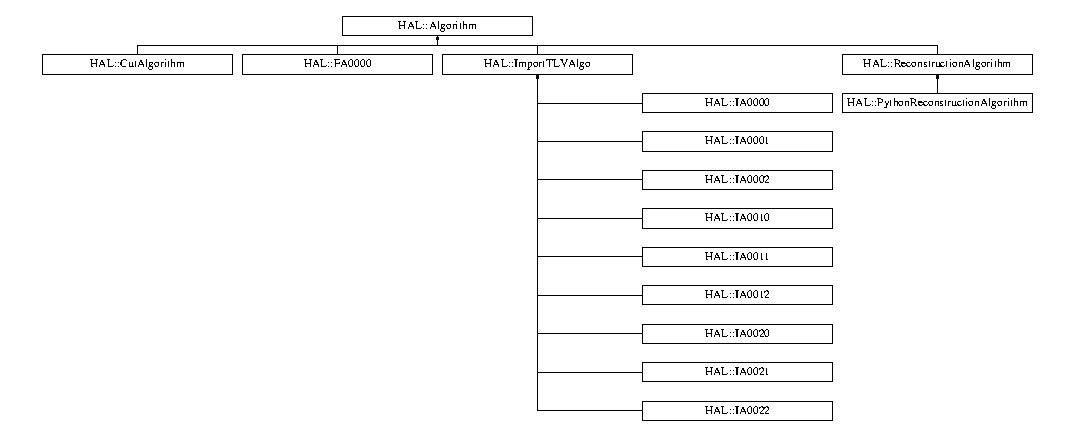
\includegraphics[height=12.000000cm]{class_h_a_l_1_1_algorithm}
\end{center}
\end{figure}
\subsection*{Public Member Functions}
\begin{DoxyCompactItemize}
\item 
\hypertarget{class_h_a_l_1_1_algorithm_a50506c07b5959ecd740f5683bf50ea93}{{\bfseries Algorithm} (T\+String name=\char`\"{}\char`\"{}, T\+String title=\char`\"{}\char`\"{})}\label{class_h_a_l_1_1_algorithm_a50506c07b5959ecd740f5683bf50ea93}

\item 
\hypertarget{class_h_a_l_1_1_algorithm_a77b66292cc2f8e021ed819daebbd7c51}{{\bfseries Algorithm} (const \hyperlink{class_h_a_l_1_1_algorithm}{Algorithm} \&algo)}\label{class_h_a_l_1_1_algorithm_a77b66292cc2f8e021ed819daebbd7c51}

\item 
\hypertarget{class_h_a_l_1_1_algorithm_a6e6834d936897cd573ce858d9b26150e}{void {\bfseries Add} (\hyperlink{class_h_a_l_1_1_algorithm}{Algorithm} $\ast$algo)}\label{class_h_a_l_1_1_algorithm_a6e6834d936897cd573ce858d9b26150e}

\item 
\hypertarget{class_h_a_l_1_1_algorithm_aaadc2f897f854c3808753fe8bdc88507}{void {\bfseries ls} ()}\label{class_h_a_l_1_1_algorithm_aaadc2f897f854c3808753fe8bdc88507}

\item 
\hypertarget{class_h_a_l_1_1_algorithm_ac6dda46e3df39cc169aaf95ced0507df}{void {\bfseries Counter\+Summary} ()}\label{class_h_a_l_1_1_algorithm_ac6dda46e3df39cc169aaf95ced0507df}

\item 
\hypertarget{class_h_a_l_1_1_algorithm_ae989038537a82ae182821bf32036a15b}{void {\bfseries Cut\+Report} ()}\label{class_h_a_l_1_1_algorithm_ae989038537a82ae182821bf32036a15b}

\item 
\hypertarget{class_h_a_l_1_1_algorithm_a5a25656c41939992b7a701f9f6c22476}{void {\bfseries Delete\+Algos} ()}\label{class_h_a_l_1_1_algorithm_a5a25656c41939992b7a701f9f6c22476}

\item 
\hypertarget{class_h_a_l_1_1_algorithm_a7815cd340c0800cd2b5567814bbcc40a}{void {\bfseries Set\+Name} (T\+String name)}\label{class_h_a_l_1_1_algorithm_a7815cd340c0800cd2b5567814bbcc40a}

\item 
\hypertarget{class_h_a_l_1_1_algorithm_aa225c7fa0c6fdef7a2807c3eaa225d83}{void {\bfseries Set\+Title} (T\+String title)}\label{class_h_a_l_1_1_algorithm_aa225c7fa0c6fdef7a2807c3eaa225d83}

\item 
\hypertarget{class_h_a_l_1_1_algorithm_ae30243bd1c0691a003d33ba6b02518cc}{void {\bfseries Set\+Output\+File\+Name} (T\+String filename)}\label{class_h_a_l_1_1_algorithm_ae30243bd1c0691a003d33ba6b02518cc}

\item 
\hypertarget{class_h_a_l_1_1_algorithm_a0b2b7e0a90824e7c2ed31fd8fc299d61}{void {\bfseries Abort} ()}\label{class_h_a_l_1_1_algorithm_a0b2b7e0a90824e7c2ed31fd8fc299d61}

\item 
\hypertarget{class_h_a_l_1_1_algorithm_a77516eeeffb62ed507616ddd006e023c}{void {\bfseries Clean\+Algos} ()}\label{class_h_a_l_1_1_algorithm_a77516eeeffb62ed507616ddd006e023c}

\item 
\hypertarget{class_h_a_l_1_1_algorithm_a64a01d69f068ef29f19057d9f4c1b172}{void {\bfseries Execute\+Algo} (Option\+\_\+t $\ast$option=\char`\"{}0\char`\"{})}\label{class_h_a_l_1_1_algorithm_a64a01d69f068ef29f19057d9f4c1b172}

\item 
\hypertarget{class_h_a_l_1_1_algorithm_aaf9d9ecdf99c327ec4de93cd5930d3c4}{void {\bfseries Execute\+Algos} (Option\+\_\+t $\ast$option)}\label{class_h_a_l_1_1_algorithm_aaf9d9ecdf99c327ec4de93cd5930d3c4}

\item 
\hypertarget{class_h_a_l_1_1_algorithm_aeb9b42850a64b3c25e7035e04c68a508}{void {\bfseries Initialize\+Algo} (Option\+\_\+t $\ast$option)}\label{class_h_a_l_1_1_algorithm_aeb9b42850a64b3c25e7035e04c68a508}

\item 
\hypertarget{class_h_a_l_1_1_algorithm_af988397097b2a83fae058744d3a909a6}{void {\bfseries Begin\+Algo} (Option\+\_\+t $\ast$option)}\label{class_h_a_l_1_1_algorithm_af988397097b2a83fae058744d3a909a6}

\item 
\hypertarget{class_h_a_l_1_1_algorithm_a82cc758128d3745ba8c91f38c4aa4d15}{void {\bfseries Slave\+Begin\+Algo} (Option\+\_\+t $\ast$option)}\label{class_h_a_l_1_1_algorithm_a82cc758128d3745ba8c91f38c4aa4d15}

\item 
\hypertarget{class_h_a_l_1_1_algorithm_a205e6c98e7b7dfca647edadaa1d159e8}{void {\bfseries Notify\+Algo} (Option\+\_\+t $\ast$option)}\label{class_h_a_l_1_1_algorithm_a205e6c98e7b7dfca647edadaa1d159e8}

\item 
\hypertarget{class_h_a_l_1_1_algorithm_ae9b629cebefe6ac8629dd6a2e66d05d6}{void {\bfseries Slave\+Terminate\+Algo} (Option\+\_\+t $\ast$option)}\label{class_h_a_l_1_1_algorithm_ae9b629cebefe6ac8629dd6a2e66d05d6}

\item 
\hypertarget{class_h_a_l_1_1_algorithm_a085a431010582d5040e51ef91e1140f1}{void {\bfseries Terminate\+Algo} (Option\+\_\+t $\ast$option)}\label{class_h_a_l_1_1_algorithm_a085a431010582d5040e51ef91e1140f1}

\item 
\hypertarget{class_h_a_l_1_1_algorithm_a7fd35cf6dc1962b58e48905b178c1747}{void {\bfseries Add\+Data} (T\+String name, T\+Object $\ast$obj)}\label{class_h_a_l_1_1_algorithm_a7fd35cf6dc1962b58e48905b178c1747}

\item 
\hypertarget{class_h_a_l_1_1_algorithm_ae9b228550b42524824f7119604df1add}{T\+Object $\ast$ {\bfseries Get\+Data} (T\+String name)}\label{class_h_a_l_1_1_algorithm_ae9b228550b42524824f7119604df1add}

\item 
\hypertarget{class_h_a_l_1_1_algorithm_a6609ea9ac6dbc42adb5b110a41201c9a}{Bool\+\_\+t {\bfseries Check\+Data} (T\+String name)}\label{class_h_a_l_1_1_algorithm_a6609ea9ac6dbc42adb5b110a41201c9a}

\item 
\hypertarget{class_h_a_l_1_1_algorithm_af0211270f880699c5a260754bbaa9640}{void {\bfseries Delete\+Data} (T\+String name)}\label{class_h_a_l_1_1_algorithm_af0211270f880699c5a260754bbaa9640}

\item 
\hypertarget{class_h_a_l_1_1_algorithm_aaae65cc70d75b35bbf4a4c987ee5fb46}{void {\bfseries Assign\+Data\+List} (T\+List $\ast$list)}\label{class_h_a_l_1_1_algorithm_aaae65cc70d75b35bbf4a4c987ee5fb46}

\item 
\hypertarget{class_h_a_l_1_1_algorithm_ae80d02cd08ddc48a82f217af77ffde20}{\hyperlink{class_h_a_l_1_1_analysis_tree_reader}{Analysis\+Tree\+Reader} $\ast$ {\bfseries Get\+Raw\+Data} ()}\label{class_h_a_l_1_1_algorithm_ae80d02cd08ddc48a82f217af77ffde20}

\item 
\hypertarget{class_h_a_l_1_1_algorithm_ae9b7d3532acfaed9b502bd462bd22c94}{\hyperlink{class_h_a_l_1_1_analysis_data}{Analysis\+Data} $\ast$ {\bfseries Get\+User\+Data} ()}\label{class_h_a_l_1_1_algorithm_ae9b7d3532acfaed9b502bd462bd22c94}

\item 
\hypertarget{class_h_a_l_1_1_algorithm_af6233cfbe13ce76207a98b12d4da6f16}{\hyperlink{class_h_a_l_1_1_analysis_tree_writer}{Analysis\+Tree\+Writer} $\ast$ {\bfseries Get\+User\+Output} ()}\label{class_h_a_l_1_1_algorithm_af6233cfbe13ce76207a98b12d4da6f16}

\item 
\hypertarget{class_h_a_l_1_1_algorithm_a0a3b6fa6eb3cf0063187c2b442f64ae8}{T\+String {\bfseries Get\+Name} ()}\label{class_h_a_l_1_1_algorithm_a0a3b6fa6eb3cf0063187c2b442f64ae8}

\item 
\hypertarget{class_h_a_l_1_1_algorithm_a9245bfda990ffdbde86cc56bcacd5b72}{T\+String {\bfseries Get\+Title} ()}\label{class_h_a_l_1_1_algorithm_a9245bfda990ffdbde86cc56bcacd5b72}

\item 
\hypertarget{class_h_a_l_1_1_algorithm_abcc3c96084def439a83bdeb0a86cb1ae}{T\+String {\bfseries Get\+Output\+File\+Name} ()}\label{class_h_a_l_1_1_algorithm_abcc3c96084def439a83bdeb0a86cb1ae}

\item 
\hypertarget{class_h_a_l_1_1_algorithm_ad5a29ecf5e77004fdd807352a15fc730}{void {\bfseries Increase\+Counter} (long long n=1)}\label{class_h_a_l_1_1_algorithm_ad5a29ecf5e77004fdd807352a15fc730}

\item 
\hypertarget{class_h_a_l_1_1_algorithm_ad155a2508e2329c4be12fbe5ec55734a}{long long {\bfseries Get\+Counter} ()}\label{class_h_a_l_1_1_algorithm_ad155a2508e2329c4be12fbe5ec55734a}

\end{DoxyCompactItemize}
\subsection*{Protected Member Functions}
\begin{DoxyCompactItemize}
\item 
\hypertarget{class_h_a_l_1_1_algorithm_a6273512af97092a7e50955cb69776d82}{virtual void {\bfseries Begin} (Option\+\_\+t $\ast$=\char`\"{}\char`\"{})}\label{class_h_a_l_1_1_algorithm_a6273512af97092a7e50955cb69776d82}

\item 
\hypertarget{class_h_a_l_1_1_algorithm_a468feb5807252729c62cce7db7d60b1d}{virtual void {\bfseries Slave\+Begin} (Option\+\_\+t $\ast$=\char`\"{}\char`\"{})}\label{class_h_a_l_1_1_algorithm_a468feb5807252729c62cce7db7d60b1d}

\item 
\hypertarget{class_h_a_l_1_1_algorithm_abe2da2ce6a2d3ccfb492d8afd1d07331}{virtual void {\bfseries Init} (Option\+\_\+t $\ast$=\char`\"{}\char`\"{})}\label{class_h_a_l_1_1_algorithm_abe2da2ce6a2d3ccfb492d8afd1d07331}

\item 
\hypertarget{class_h_a_l_1_1_algorithm_acbbfee57e6c71ab04047dca6636f2c4f}{virtual void {\bfseries Notify} (Option\+\_\+t $\ast$=\char`\"{}\char`\"{})}\label{class_h_a_l_1_1_algorithm_acbbfee57e6c71ab04047dca6636f2c4f}

\item 
\hypertarget{class_h_a_l_1_1_algorithm_a438c5c54698aa014b660474d08703bc2}{virtual void {\bfseries Exec} (Option\+\_\+t $\ast$=\char`\"{}\char`\"{})}\label{class_h_a_l_1_1_algorithm_a438c5c54698aa014b660474d08703bc2}

\item 
\hypertarget{class_h_a_l_1_1_algorithm_a2a26a5549e92efaa968763ac51e6758a}{virtual void {\bfseries Clear} (Option\+\_\+t $\ast$=\char`\"{}\char`\"{})}\label{class_h_a_l_1_1_algorithm_a2a26a5549e92efaa968763ac51e6758a}

\item 
\hypertarget{class_h_a_l_1_1_algorithm_a9735cc4d7ef34d440aff116c8dbf5cbb}{virtual void {\bfseries Slave\+Terminate} (Option\+\_\+t $\ast$=\char`\"{}\char`\"{})}\label{class_h_a_l_1_1_algorithm_a9735cc4d7ef34d440aff116c8dbf5cbb}

\item 
\hypertarget{class_h_a_l_1_1_algorithm_ab974f3b6336b7b1002c72c04ad2b59cb}{virtual void {\bfseries Terminate} (Option\+\_\+t $\ast$=\char`\"{}\char`\"{})}\label{class_h_a_l_1_1_algorithm_ab974f3b6336b7b1002c72c04ad2b59cb}

\end{DoxyCompactItemize}
\subsection*{Protected Attributes}
\begin{DoxyCompactItemize}
\item 
\hypertarget{class_h_a_l_1_1_algorithm_aacc4824bcc223fc86f0f57662393e56c}{T\+List $\ast$ {\bfseries f\+Data\+List}}\label{class_h_a_l_1_1_algorithm_aacc4824bcc223fc86f0f57662393e56c}

\item 
\hypertarget{class_h_a_l_1_1_algorithm_a15bbd1834a2413957b2946e051584d49}{T\+String {\bfseries f\+Algorithm\+Type}}\label{class_h_a_l_1_1_algorithm_a15bbd1834a2413957b2946e051584d49}

\item 
\hypertarget{class_h_a_l_1_1_algorithm_a91a834bebb25ccc2e4324fcaf51bf294}{long long {\bfseries f\+Counter}}\label{class_h_a_l_1_1_algorithm_a91a834bebb25ccc2e4324fcaf51bf294}

\end{DoxyCompactItemize}


The documentation for this class was generated from the following file\+:\begin{DoxyCompactItemize}
\item 
/\+Users/jhetherly/src/root\+\_\+\+H\+A\+L/include/\+H\+A\+L/Algorithm.\+h\end{DoxyCompactItemize}

\hypertarget{class_h_a_l_1_1_analysis}{\section{H\-A\-L\-:\-:Analysis Class Reference}
\label{class_h_a_l_1_1_analysis}\index{H\-A\-L\-::\-Analysis@{H\-A\-L\-::\-Analysis}}
}
\subsection*{Public Member Functions}
\begin{DoxyCompactItemize}
\item 
\hypertarget{class_h_a_l_1_1_analysis_ab95bfff098f6a9543d444078cef3be91}{{\bfseries Analysis} (T\-String name=\char`\"{}\char`\"{}, T\-String title=\char`\"{}\char`\"{}, T\-String tree\-Name=\char`\"{}\char`\"{})}\label{class_h_a_l_1_1_analysis_ab95bfff098f6a9543d444078cef3be91}

\item 
\hypertarget{class_h_a_l_1_1_analysis_ac7e8314701f2b10f684d3b795031299e}{void {\bfseries Add\-Reco\-Algo} (\hyperlink{class_h_a_l_1_1_algorithm}{Algorithm} $\ast$r)}\label{class_h_a_l_1_1_analysis_ac7e8314701f2b10f684d3b795031299e}

\item 
\hypertarget{class_h_a_l_1_1_analysis_a4cdeca8d55dbfcc19261baedca02e424}{void {\bfseries Add\-Cut\-Algo} (\hyperlink{class_h_a_l_1_1_algorithm}{Algorithm} $\ast$c)}\label{class_h_a_l_1_1_analysis_a4cdeca8d55dbfcc19261baedca02e424}

\item 
\hypertarget{class_h_a_l_1_1_analysis_af755ad7b542eb634144c99b1d142519c}{void {\bfseries Print\-Analysis\-Flow} ()}\label{class_h_a_l_1_1_analysis_af755ad7b542eb634144c99b1d142519c}

\item 
\hypertarget{class_h_a_l_1_1_analysis_a56e97ef132e10b2a5f96c71c5145127b}{void {\bfseries Set\-Tree\-Object\-Name} (T\-String name)}\label{class_h_a_l_1_1_analysis_a56e97ef132e10b2a5f96c71c5145127b}

\item 
\hypertarget{class_h_a_l_1_1_analysis_abcbdb0f6cad2060cf3f6bca7d0eb9ada}{void {\bfseries Set\-Analysis\-Name} (T\-String name)}\label{class_h_a_l_1_1_analysis_abcbdb0f6cad2060cf3f6bca7d0eb9ada}

\item 
\hypertarget{class_h_a_l_1_1_analysis_ab4ecf4f7c5c29027ac3eb3e3a2e3a780}{void {\bfseries Set\-Analysis\-Title} (T\-String title)}\label{class_h_a_l_1_1_analysis_ab4ecf4f7c5c29027ac3eb3e3a2e3a780}

\item 
\hypertarget{class_h_a_l_1_1_analysis_a540cf522be42290e16d6ac0c7dbff0ba}{Int\-\_\-t {\bfseries Add\-Files} (T\-String fnames, Long64\-\_\-t nentries=1234567890)}\label{class_h_a_l_1_1_analysis_a540cf522be42290e16d6ac0c7dbff0ba}

\item 
\hypertarget{class_h_a_l_1_1_analysis_af8fccc1f3c27d6402ecad559648b7ff0}{Int\-\_\-t {\bfseries Add\-Files} (T\-Chain $\ast$fchain)}\label{class_h_a_l_1_1_analysis_af8fccc1f3c27d6402ecad559648b7ff0}

\item 
\hypertarget{class_h_a_l_1_1_analysis_a9e6b12787599c0c36f576350e2e93b8d}{void {\bfseries Set\-Output\-File\-Name} (T\-String fname)}\label{class_h_a_l_1_1_analysis_a9e6b12787599c0c36f576350e2e93b8d}

\item 
\hypertarget{class_h_a_l_1_1_analysis_a50f84d17528b7ba7621c65696dd81e75}{void {\bfseries Set\-Output\-Tree\-Name} (T\-String tname)}\label{class_h_a_l_1_1_analysis_a50f84d17528b7ba7621c65696dd81e75}

\item 
\hypertarget{class_h_a_l_1_1_analysis_a6461758cc06f7a334a487d857172983a}{void {\bfseries Set\-Output\-Tree\-Description} (T\-String tdescription)}\label{class_h_a_l_1_1_analysis_a6461758cc06f7a334a487d857172983a}

\item 
\hypertarget{class_h_a_l_1_1_analysis_afccfbae795035cfe75578fa805aefa93}{void {\bfseries Print\-Tree} (Option\-\_\-t $\ast$option=\char`\"{}\char`\"{})}\label{class_h_a_l_1_1_analysis_afccfbae795035cfe75578fa805aefa93}

\item 
\hypertarget{class_h_a_l_1_1_analysis_a7c6603a4cc7b74591f5c0427f59023d5}{const char $\ast$ {\bfseries Get\-Leaf\-Type} (T\-String leafname)}\label{class_h_a_l_1_1_analysis_a7c6603a4cc7b74591f5c0427f59023d5}

\item 
\hypertarget{class_h_a_l_1_1_analysis_a8410426a53f7828270531f1ec56340b8}{const char $\ast$ {\bfseries Get\-Leaf\-Type} (T\-String branchname, T\-String leafname)}\label{class_h_a_l_1_1_analysis_a8410426a53f7828270531f1ec56340b8}

\item 
\hypertarget{class_h_a_l_1_1_analysis_a6e11fa65e712377587ed4b6a1a62c8aa}{void {\bfseries Map\-Branch} (T\-String branchname, T\-String nickname)}\label{class_h_a_l_1_1_analysis_a6e11fa65e712377587ed4b6a1a62c8aa}

\item 
\hypertarget{class_h_a_l_1_1_analysis_a4278a2e961076913371dec71da389701}{Long64\-\_\-t {\bfseries Process} (Option\-\_\-t $\ast$option=\char`\"{}\char`\"{}, Long64\-\_\-t nentries=1234567890, Long64\-\_\-t firstentry=0)}\label{class_h_a_l_1_1_analysis_a4278a2e961076913371dec71da389701}

\end{DoxyCompactItemize}


The documentation for this class was generated from the following file\-:\begin{DoxyCompactItemize}
\item 
/\-Users/jhetherly/src/root\-\_\-\-H\-A\-L/include/\-H\-A\-L/Analysis.\-h\end{DoxyCompactItemize}

\hypertarget{class_h_a_l_1_1_analysis_data}{\section{H\-A\-L\-:\-:Analysis\-Data Class Reference}
\label{class_h_a_l_1_1_analysis_data}\index{H\-A\-L\-::\-Analysis\-Data@{H\-A\-L\-::\-Analysis\-Data}}
}
Inheritance diagram for H\-A\-L\-:\-:Analysis\-Data\-:\begin{figure}[H]
\begin{center}
\leavevmode
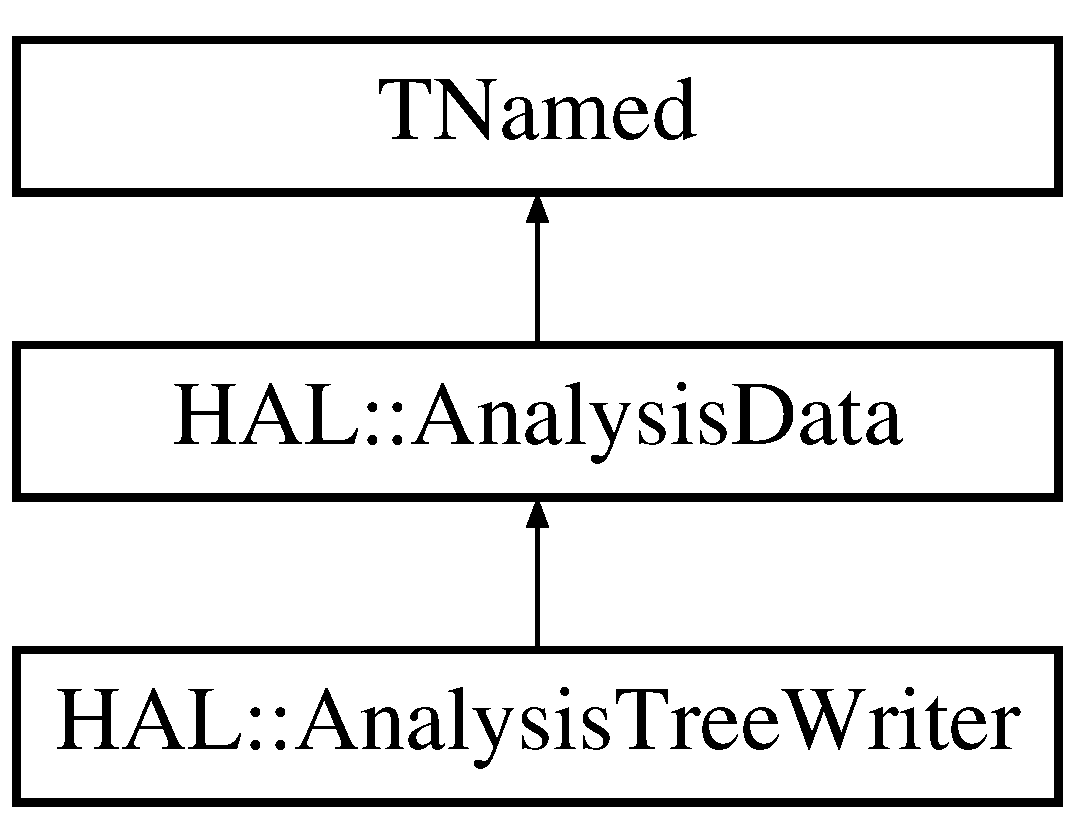
\includegraphics[height=3.000000cm]{class_h_a_l_1_1_analysis_data}
\end{center}
\end{figure}
\subsection*{Public Member Functions}
\begin{DoxyCompactItemize}
\item 
\hypertarget{class_h_a_l_1_1_analysis_data_a3870a72f6b39f3b4509b2498d285d94a}{virtual void {\bfseries Set\-Value} (const T\-String \&, const bool \&)}\label{class_h_a_l_1_1_analysis_data_a3870a72f6b39f3b4509b2498d285d94a}

\item 
\hypertarget{class_h_a_l_1_1_analysis_data_af74aff588a73f1c4d0a5e5ecbad14efb}{virtual void {\bfseries Set\-Value} (const T\-String \&, const long double \&)}\label{class_h_a_l_1_1_analysis_data_af74aff588a73f1c4d0a5e5ecbad14efb}

\item 
\hypertarget{class_h_a_l_1_1_analysis_data_ae88cc39a2594cf0bb969e3626cf17412}{virtual void {\bfseries Set\-Value} (const T\-String n, const double \&v)}\label{class_h_a_l_1_1_analysis_data_ae88cc39a2594cf0bb969e3626cf17412}

\item 
\hypertarget{class_h_a_l_1_1_analysis_data_a3953675a3b647f8c87eb214e25940d77}{virtual void {\bfseries Set\-Value} (const T\-String \&n, const float \&v)}\label{class_h_a_l_1_1_analysis_data_a3953675a3b647f8c87eb214e25940d77}

\item 
\hypertarget{class_h_a_l_1_1_analysis_data_ad18a729c4979bacc30d32e0802520236}{virtual void {\bfseries Set\-Value} (const T\-String \&, const long long \&)}\label{class_h_a_l_1_1_analysis_data_ad18a729c4979bacc30d32e0802520236}

\item 
\hypertarget{class_h_a_l_1_1_analysis_data_a2d3510dc4ee329387906e8738061b6b4}{virtual void {\bfseries Set\-Value} (const T\-String \&n, const short \&v)}\label{class_h_a_l_1_1_analysis_data_a2d3510dc4ee329387906e8738061b6b4}

\item 
\hypertarget{class_h_a_l_1_1_analysis_data_af8f2df54ad897dce65aa6224cac0af7c}{virtual void {\bfseries Set\-Value} (const T\-String \&n, const long \&v)}\label{class_h_a_l_1_1_analysis_data_af8f2df54ad897dce65aa6224cac0af7c}

\item 
\hypertarget{class_h_a_l_1_1_analysis_data_a697cb757197048cbcc5716bb32499c60}{virtual void {\bfseries Set\-Value} (const T\-String \&n, const int \&v)}\label{class_h_a_l_1_1_analysis_data_a697cb757197048cbcc5716bb32499c60}

\item 
\hypertarget{class_h_a_l_1_1_analysis_data_ae248b4f6c90034c9a41f8f8618ed89b8}{virtual void {\bfseries Set\-Value} (const T\-String \&n, const signed char \&v)}\label{class_h_a_l_1_1_analysis_data_ae248b4f6c90034c9a41f8f8618ed89b8}

\item 
\hypertarget{class_h_a_l_1_1_analysis_data_a0d21eebe0e1566531fa5c736f2cc6ed2}{virtual void {\bfseries Set\-Value} (const T\-String \&, const unsigned long long \&)}\label{class_h_a_l_1_1_analysis_data_a0d21eebe0e1566531fa5c736f2cc6ed2}

\item 
\hypertarget{class_h_a_l_1_1_analysis_data_a08be235fce5fd10cfafc592a2d9c1448}{virtual void {\bfseries Set\-Value} (const T\-String \&n, const unsigned short \&v)}\label{class_h_a_l_1_1_analysis_data_a08be235fce5fd10cfafc592a2d9c1448}

\item 
\hypertarget{class_h_a_l_1_1_analysis_data_af9cca2f941fef23004516aefc0d9c00d}{virtual void {\bfseries Set\-Value} (const T\-String \&n, const unsigned long \&v)}\label{class_h_a_l_1_1_analysis_data_af9cca2f941fef23004516aefc0d9c00d}

\item 
\hypertarget{class_h_a_l_1_1_analysis_data_adac44d46dc879cda67371131c18cf233}{virtual void {\bfseries Set\-Value} (const T\-String \&n, const unsigned int \&v)}\label{class_h_a_l_1_1_analysis_data_adac44d46dc879cda67371131c18cf233}

\item 
\hypertarget{class_h_a_l_1_1_analysis_data_ab3237d1010394bff323821642ea2380c}{virtual void {\bfseries Set\-Value} (const T\-String \&n, const unsigned char \&v)}\label{class_h_a_l_1_1_analysis_data_ab3237d1010394bff323821642ea2380c}

\item 
\hypertarget{class_h_a_l_1_1_analysis_data_a3fcb628c26524a1cc11db49295581d2d}{virtual void {\bfseries Set\-Value} (const T\-String \&n, const std\-::string \&v)}\label{class_h_a_l_1_1_analysis_data_a3fcb628c26524a1cc11db49295581d2d}

\item 
\hypertarget{class_h_a_l_1_1_analysis_data_acb8dd69db78b9d748ad4966584c7fa78}{virtual void {\bfseries Set\-Value} (const T\-String \&n, const T\-String \&v)}\label{class_h_a_l_1_1_analysis_data_acb8dd69db78b9d748ad4966584c7fa78}

\item 
\hypertarget{class_h_a_l_1_1_analysis_data_a7ffd3d35192f72eeadb3274a9bf8694d}{virtual void {\bfseries Set\-Value} (const T\-String \&n, const char \&v)}\label{class_h_a_l_1_1_analysis_data_a7ffd3d35192f72eeadb3274a9bf8694d}

\item 
\hypertarget{class_h_a_l_1_1_analysis_data_ac30be252a2ee9afe72db28b4cc2160da}{virtual void {\bfseries Set\-Value} (const T\-String \&, T\-Object $\ast$)}\label{class_h_a_l_1_1_analysis_data_ac30be252a2ee9afe72db28b4cc2160da}

\item 
\hypertarget{class_h_a_l_1_1_analysis_data_a12ad774235747ddc93efe315b22bf9e6}{virtual void {\bfseries Set\-Value} (const T\-String \&, const bool \&, const long long \&)}\label{class_h_a_l_1_1_analysis_data_a12ad774235747ddc93efe315b22bf9e6}

\item 
\hypertarget{class_h_a_l_1_1_analysis_data_a2628f2b892533b16f0a991bee3e0054b}{virtual void {\bfseries Set\-Value} (const T\-String \&, const long double \&, const long long \&)}\label{class_h_a_l_1_1_analysis_data_a2628f2b892533b16f0a991bee3e0054b}

\item 
\hypertarget{class_h_a_l_1_1_analysis_data_a59a7de41ba6832fb70f97b4c1e275fd3}{virtual void {\bfseries Set\-Value} (const T\-String \&n, const double \&v, const long long \&i)}\label{class_h_a_l_1_1_analysis_data_a59a7de41ba6832fb70f97b4c1e275fd3}

\item 
\hypertarget{class_h_a_l_1_1_analysis_data_a69059a19ae4a37a01eedfa98c537c487}{virtual void {\bfseries Set\-Value} (const T\-String \&n, const float \&v, const long long \&i)}\label{class_h_a_l_1_1_analysis_data_a69059a19ae4a37a01eedfa98c537c487}

\item 
\hypertarget{class_h_a_l_1_1_analysis_data_aad5a01dc8b2510bdcb47854a3cdaba0d}{virtual void {\bfseries Set\-Value} (const T\-String \&, const long long \&, const long long \&)}\label{class_h_a_l_1_1_analysis_data_aad5a01dc8b2510bdcb47854a3cdaba0d}

\item 
\hypertarget{class_h_a_l_1_1_analysis_data_adfb861d9e83e6880e54d11447b7047be}{virtual void {\bfseries Set\-Value} (const T\-String \&n, const short \&v, const long long \&i)}\label{class_h_a_l_1_1_analysis_data_adfb861d9e83e6880e54d11447b7047be}

\item 
\hypertarget{class_h_a_l_1_1_analysis_data_ac01b1d8a623777b81d5969d2b553a003}{virtual void {\bfseries Set\-Value} (const T\-String \&n, const long \&v, const long long \&i)}\label{class_h_a_l_1_1_analysis_data_ac01b1d8a623777b81d5969d2b553a003}

\item 
\hypertarget{class_h_a_l_1_1_analysis_data_aaddff4f1a41b2311b5f59a4eb4eb7a41}{virtual void {\bfseries Set\-Value} (const T\-String \&n, const int \&v, const long long \&i)}\label{class_h_a_l_1_1_analysis_data_aaddff4f1a41b2311b5f59a4eb4eb7a41}

\item 
\hypertarget{class_h_a_l_1_1_analysis_data_acea99cc8c68cf2a9d5f82da7e0d33202}{virtual void {\bfseries Set\-Value} (const T\-String \&n, const signed char \&v, const long long \&i)}\label{class_h_a_l_1_1_analysis_data_acea99cc8c68cf2a9d5f82da7e0d33202}

\item 
\hypertarget{class_h_a_l_1_1_analysis_data_a20938ad3fcd255b41f894e44b3e363f8}{virtual void {\bfseries Set\-Value} (const T\-String \&, const unsigned long long \&, const long long \&)}\label{class_h_a_l_1_1_analysis_data_a20938ad3fcd255b41f894e44b3e363f8}

\item 
\hypertarget{class_h_a_l_1_1_analysis_data_a8d61e54fe6022a58837468e1059a7e80}{virtual void {\bfseries Set\-Value} (const T\-String \&n, const unsigned short \&v, const long long \&i)}\label{class_h_a_l_1_1_analysis_data_a8d61e54fe6022a58837468e1059a7e80}

\item 
\hypertarget{class_h_a_l_1_1_analysis_data_a2af1428a8feebf6769cb30dd656d4b1e}{virtual void {\bfseries Set\-Value} (const T\-String \&n, const unsigned long \&v, const long long \&i)}\label{class_h_a_l_1_1_analysis_data_a2af1428a8feebf6769cb30dd656d4b1e}

\item 
\hypertarget{class_h_a_l_1_1_analysis_data_a446ed8d103e405b5028a9cebeae11bdf}{virtual void {\bfseries Set\-Value} (const T\-String \&n, const unsigned int \&v, const long long \&i)}\label{class_h_a_l_1_1_analysis_data_a446ed8d103e405b5028a9cebeae11bdf}

\item 
\hypertarget{class_h_a_l_1_1_analysis_data_af11d8522043ee9ddebea6beddfafdb1f}{virtual void {\bfseries Set\-Value} (const T\-String \&n, const unsigned char \&v, const long long \&i)}\label{class_h_a_l_1_1_analysis_data_af11d8522043ee9ddebea6beddfafdb1f}

\item 
\hypertarget{class_h_a_l_1_1_analysis_data_a2c1fe18ae83a39d8278630896e3b20cf}{virtual void {\bfseries Set\-Value} (const T\-String \&, const std\-::string \&, const long long \&)}\label{class_h_a_l_1_1_analysis_data_a2c1fe18ae83a39d8278630896e3b20cf}

\item 
\hypertarget{class_h_a_l_1_1_analysis_data_a985317d132d7c150e61f869db7fa8197}{virtual void {\bfseries Set\-Value} (const T\-String \&n, const T\-String \&v, const long long \&i)}\label{class_h_a_l_1_1_analysis_data_a985317d132d7c150e61f869db7fa8197}

\item 
\hypertarget{class_h_a_l_1_1_analysis_data_ae67a81418f6b826dd9b04f4c1e6f6f43}{virtual void {\bfseries Set\-Value} (const T\-String \&n, const char \&v, const long long \&i)}\label{class_h_a_l_1_1_analysis_data_ae67a81418f6b826dd9b04f4c1e6f6f43}

\item 
\hypertarget{class_h_a_l_1_1_analysis_data_adb01a8781d1c24a520bcc1b2518b64d2}{virtual void {\bfseries Set\-Value} (const T\-String \&, T\-Object $\ast$, const long long \&)}\label{class_h_a_l_1_1_analysis_data_adb01a8781d1c24a520bcc1b2518b64d2}

\item 
\hypertarget{class_h_a_l_1_1_analysis_data_a8d9a745e5e829f20b1e2e5fd5651b5cb}{virtual void {\bfseries Set\-Value} (const T\-String \&, const bool \&, const long long \&, const long long \&)}\label{class_h_a_l_1_1_analysis_data_a8d9a745e5e829f20b1e2e5fd5651b5cb}

\item 
\hypertarget{class_h_a_l_1_1_analysis_data_ad81a9423de201ecd3993c69c4cbefe6c}{virtual void {\bfseries Set\-Value} (const T\-String \&, const long double \&, const long long \&, const long long \&)}\label{class_h_a_l_1_1_analysis_data_ad81a9423de201ecd3993c69c4cbefe6c}

\item 
\hypertarget{class_h_a_l_1_1_analysis_data_a53d8939f8a64262857f13025f1f040da}{virtual void {\bfseries Set\-Value} (const T\-String \&n, const double \&v, const long long \&i, const long long \&j)}\label{class_h_a_l_1_1_analysis_data_a53d8939f8a64262857f13025f1f040da}

\item 
\hypertarget{class_h_a_l_1_1_analysis_data_a0089459ec31db3ea3c5dd974502ba651}{virtual void {\bfseries Set\-Value} (const T\-String \&n, const float \&v, const long long \&i, const long long \&j)}\label{class_h_a_l_1_1_analysis_data_a0089459ec31db3ea3c5dd974502ba651}

\item 
\hypertarget{class_h_a_l_1_1_analysis_data_a04aaec235f3100f4324bc502764fe00f}{virtual void {\bfseries Set\-Value} (const T\-String \&, const long long \&, const long long \&, const long long \&)}\label{class_h_a_l_1_1_analysis_data_a04aaec235f3100f4324bc502764fe00f}

\item 
\hypertarget{class_h_a_l_1_1_analysis_data_ad17c472ec1b6a6a0259c26bc5e1d68a9}{virtual void {\bfseries Set\-Value} (const T\-String \&n, const short \&v, const long long \&i, const long long \&j)}\label{class_h_a_l_1_1_analysis_data_ad17c472ec1b6a6a0259c26bc5e1d68a9}

\item 
\hypertarget{class_h_a_l_1_1_analysis_data_a4ab8550b85c33c0d04fcc381c845a5c4}{virtual void {\bfseries Set\-Value} (const T\-String \&n, const long \&v, const long long \&i, const long long \&j)}\label{class_h_a_l_1_1_analysis_data_a4ab8550b85c33c0d04fcc381c845a5c4}

\item 
\hypertarget{class_h_a_l_1_1_analysis_data_a9e7eea804e43369c4a4a8c3b1dacad37}{virtual void {\bfseries Set\-Value} (const T\-String \&n, const int \&v, const long long \&i, const long long \&j)}\label{class_h_a_l_1_1_analysis_data_a9e7eea804e43369c4a4a8c3b1dacad37}

\item 
\hypertarget{class_h_a_l_1_1_analysis_data_aebc6089b43396b0f19c1e06862be5448}{virtual void {\bfseries Set\-Value} (const T\-String \&n, const signed char \&v, const long long \&i, const long long \&j)}\label{class_h_a_l_1_1_analysis_data_aebc6089b43396b0f19c1e06862be5448}

\item 
\hypertarget{class_h_a_l_1_1_analysis_data_ae89756ae4ac0bf7cffbd22fbb54a2ec0}{virtual void {\bfseries Set\-Value} (const T\-String \&, const unsigned long long \&, const long long \&, const long long \&)}\label{class_h_a_l_1_1_analysis_data_ae89756ae4ac0bf7cffbd22fbb54a2ec0}

\item 
\hypertarget{class_h_a_l_1_1_analysis_data_a3f98354687b412c2fb8e84615211d314}{virtual void {\bfseries Set\-Value} (const T\-String \&n, const unsigned short \&v, const long long \&i, const long long \&j)}\label{class_h_a_l_1_1_analysis_data_a3f98354687b412c2fb8e84615211d314}

\item 
\hypertarget{class_h_a_l_1_1_analysis_data_af569db19521306fa14e85bd9d784a17f}{virtual void {\bfseries Set\-Value} (const T\-String \&n, const unsigned long \&v, const long long \&i, const long long \&j)}\label{class_h_a_l_1_1_analysis_data_af569db19521306fa14e85bd9d784a17f}

\item 
\hypertarget{class_h_a_l_1_1_analysis_data_a9c57d185dc584fdfb7f38b86e5f47f53}{virtual void {\bfseries Set\-Value} (const T\-String \&n, const unsigned int \&v, const long long \&i, const long long \&j)}\label{class_h_a_l_1_1_analysis_data_a9c57d185dc584fdfb7f38b86e5f47f53}

\item 
\hypertarget{class_h_a_l_1_1_analysis_data_a976258cc088753ba46ddad2b89bec07a}{virtual void {\bfseries Set\-Value} (const T\-String \&n, const unsigned char \&v, const long long \&i, const long long \&j)}\label{class_h_a_l_1_1_analysis_data_a976258cc088753ba46ddad2b89bec07a}

\item 
\hypertarget{class_h_a_l_1_1_analysis_data_a3782d0d87d85a96370d1c1b26523bc7e}{virtual void {\bfseries Set\-Value} (const T\-String \&, const std\-::string \&, const long long \&, const long long \&)}\label{class_h_a_l_1_1_analysis_data_a3782d0d87d85a96370d1c1b26523bc7e}

\item 
\hypertarget{class_h_a_l_1_1_analysis_data_a6cc252333af3e3c425ad4a184f286816}{virtual void {\bfseries Set\-Value} (const T\-String \&n, const T\-String \&v, const long long \&i, const long long \&j)}\label{class_h_a_l_1_1_analysis_data_a6cc252333af3e3c425ad4a184f286816}

\item 
\hypertarget{class_h_a_l_1_1_analysis_data_a7ce85e90fa181f17d72476422da24a48}{virtual void {\bfseries Set\-Value} (const T\-String \&n, const char \&v, const long long \&i, const long long \&j)}\label{class_h_a_l_1_1_analysis_data_a7ce85e90fa181f17d72476422da24a48}

\item 
\hypertarget{class_h_a_l_1_1_analysis_data_aedeeb6d1ff74a47232f5cb33edfbd88c}{virtual void {\bfseries Set\-Value} (const T\-String \&, T\-Object $\ast$, const long long \&, const long long \&)}\label{class_h_a_l_1_1_analysis_data_aedeeb6d1ff74a47232f5cb33edfbd88c}

\item 
\hypertarget{class_h_a_l_1_1_analysis_data_a281cfe7bf707071ac81004f415842f50}{bool {\bfseries Get\-Bool} (const T\-String \&, const long long \&i=-\/1, const long long \&j=-\/1)}\label{class_h_a_l_1_1_analysis_data_a281cfe7bf707071ac81004f415842f50}

\item 
\hypertarget{class_h_a_l_1_1_analysis_data_aab51c395613c253b5bdd019eb72a78dc}{long double {\bfseries Get\-Decimal} (const T\-String \&, const long long \&i=-\/1, const long long \&j=-\/1)}\label{class_h_a_l_1_1_analysis_data_aab51c395613c253b5bdd019eb72a78dc}

\item 
\hypertarget{class_h_a_l_1_1_analysis_data_a4695a073f8dc031fd3f0c0c2d6d4a64e}{long long {\bfseries Get\-Integer} (const T\-String \&, const long long \&i=-\/1, const long long \&j=-\/1)}\label{class_h_a_l_1_1_analysis_data_a4695a073f8dc031fd3f0c0c2d6d4a64e}

\item 
\hypertarget{class_h_a_l_1_1_analysis_data_af7d47f613b3745eae74b59e82d718b5b}{unsigned long long {\bfseries Get\-Counting} (const T\-String \&, const long long \&i=-\/1, const long long \&j=-\/1)}\label{class_h_a_l_1_1_analysis_data_af7d47f613b3745eae74b59e82d718b5b}

\item 
\hypertarget{class_h_a_l_1_1_analysis_data_a983d806a18f7d81bf7b0405375442e9d}{T\-String {\bfseries Get\-String} (const T\-String \&, const long long \&i=-\/1, const long long \&j=-\/1)}\label{class_h_a_l_1_1_analysis_data_a983d806a18f7d81bf7b0405375442e9d}

\item 
\hypertarget{class_h_a_l_1_1_analysis_data_af1d5b191d8ccec6fb120a7debee1a474}{T\-Object $\ast$ {\bfseries Get\-T\-Object} (const T\-String \&, const long long \&i=-\/1, const long long \&j=-\/1)}\label{class_h_a_l_1_1_analysis_data_af1d5b191d8ccec6fb120a7debee1a474}

\item 
\hypertarget{class_h_a_l_1_1_analysis_data_a88485900b08fc820b2021234699d72d9}{bool {\bfseries Exists} (const T\-String \&n, const long long \&i=-\/1, const long long \&j=-\/1)}\label{class_h_a_l_1_1_analysis_data_a88485900b08fc820b2021234699d72d9}

\item 
\hypertarget{class_h_a_l_1_1_analysis_data_a493762f931219f8a720d06a263a4ad23}{unsigned {\bfseries Type\-Dim} (std\-::string n)}\label{class_h_a_l_1_1_analysis_data_a493762f931219f8a720d06a263a4ad23}

\item 
\hypertarget{class_h_a_l_1_1_analysis_data_ab0c4af2c4db8ebe38fd883ed0a2c2a72}{unsigned {\bfseries Type\-Dim} (const T\-String \&n)}\label{class_h_a_l_1_1_analysis_data_ab0c4af2c4db8ebe38fd883ed0a2c2a72}

\item 
\hypertarget{class_h_a_l_1_1_analysis_data_ae12492f13299eabe287205392489a4c4}{std\-::vector$<$ T\-String $>$ {\bfseries Get\-Similar\-Names} (const T\-String \&n, unsigned min\-\_\-dim)}\label{class_h_a_l_1_1_analysis_data_ae12492f13299eabe287205392489a4c4}

\item 
\hypertarget{class_h_a_l_1_1_analysis_data_a02f185a0bb593efe8f1e1605a8db7212}{void {\bfseries Copy\-Values} (const T\-String \&from, const T\-String \&to)}\label{class_h_a_l_1_1_analysis_data_a02f185a0bb593efe8f1e1605a8db7212}

\item 
\hypertarget{class_h_a_l_1_1_analysis_data_a44bfe71b3f3c88ce664e6d7b3bd9b111}{void {\bfseries Swap\-Values} (const T\-String \&n, long long i, long long j)}\label{class_h_a_l_1_1_analysis_data_a44bfe71b3f3c88ce664e6d7b3bd9b111}

\item 
\hypertarget{class_h_a_l_1_1_analysis_data_add418841a62be11aad64044e7eda5ffb}{void {\bfseries Reset} ()}\label{class_h_a_l_1_1_analysis_data_add418841a62be11aad64044e7eda5ffb}

\item 
\hypertarget{class_h_a_l_1_1_analysis_data_a39276ed7623a74cf6468fa9a69079e07}{void {\bfseries Remove\-Name\-And\-Data} (const T\-String \&)}\label{class_h_a_l_1_1_analysis_data_a39276ed7623a74cf6468fa9a69079e07}

\item 
\hypertarget{class_h_a_l_1_1_analysis_data_a35cbc682e6090bf2540ac62de07db82f}{void {\bfseries Remove\-Data} (const T\-String \&)}\label{class_h_a_l_1_1_analysis_data_a35cbc682e6090bf2540ac62de07db82f}

\item 
\hypertarget{class_h_a_l_1_1_analysis_data_a9e60f6b78b29280597ac991cf378f4f3}{void {\bfseries Remove\-All\-Associated\-Data} (const T\-String \&)}\label{class_h_a_l_1_1_analysis_data_a9e60f6b78b29280597ac991cf378f4f3}

\item 
\hypertarget{class_h_a_l_1_1_analysis_data_a0d63364d678190ac69e46922ad445b8a}{{\bfseries Class\-Def\-N\-V} (\hyperlink{class_h_a_l_1_1_analysis_data}{Analysis\-Data}, 0)}\label{class_h_a_l_1_1_analysis_data_a0d63364d678190ac69e46922ad445b8a}

\end{DoxyCompactItemize}
\subsection*{Public Attributes}
\begin{DoxyCompactItemize}
\item 
\hypertarget{class_h_a_l_1_1_analysis_data_adc7232f1a112de23d2b557740422ec9f}{std\-::map$<$ std\-::string, bool, \\*
internal\-::string\-\_\-cmp $>$ {\bfseries f\-Bool\-Map}}\label{class_h_a_l_1_1_analysis_data_adc7232f1a112de23d2b557740422ec9f}

\item 
\hypertarget{class_h_a_l_1_1_analysis_data_a79170e31902d40d73d6838b816e74dc8}{std\-::map$<$ std\-::string, long \\*
double, internal\-::string\-\_\-cmp $>$ {\bfseries f\-Decimal\-Map}}\label{class_h_a_l_1_1_analysis_data_a79170e31902d40d73d6838b816e74dc8}

\item 
\hypertarget{class_h_a_l_1_1_analysis_data_a5487671b851b8ce89298d7f770ab8f34}{std\-::map$<$ std\-::string, long \\*
long, internal\-::string\-\_\-cmp $>$ {\bfseries f\-Integer\-Map}}\label{class_h_a_l_1_1_analysis_data_a5487671b851b8ce89298d7f770ab8f34}

\item 
\hypertarget{class_h_a_l_1_1_analysis_data_a6f29542f7f2cd7e7377c56ac54592dd5}{std\-::map$<$ std\-::string, \\*
unsigned long long, \\*
internal\-::string\-\_\-cmp $>$ {\bfseries f\-Counting\-Map}}\label{class_h_a_l_1_1_analysis_data_a6f29542f7f2cd7e7377c56ac54592dd5}

\item 
\hypertarget{class_h_a_l_1_1_analysis_data_a3256b3efc77655ba25cc34a6986c00d5}{std\-::map$<$ std\-::string, \\*
std\-::string, \\*
internal\-::string\-\_\-cmp $>$ {\bfseries f\-String\-Map}}\label{class_h_a_l_1_1_analysis_data_a3256b3efc77655ba25cc34a6986c00d5}

\item 
\hypertarget{class_h_a_l_1_1_analysis_data_a913d66198c57cc2bd9f0e3e5d904e33f}{std\-::map$<$ std\-::string, T\-Object \\*
$\ast$, internal\-::string\-\_\-cmp $>$ {\bfseries f\-T\-Object\-Map}}\label{class_h_a_l_1_1_analysis_data_a913d66198c57cc2bd9f0e3e5d904e33f}

\item 
\hypertarget{class_h_a_l_1_1_analysis_data_a61184b1f5c3fe3a707ca6636ae9e13b0}{std\-::map$<$ std\-::string, \\*
std\-::map$<$ long long, bool $>$\\*
, internal\-::string\-\_\-cmp $>$ {\bfseries f\-Bool\-Int\-Map}}\label{class_h_a_l_1_1_analysis_data_a61184b1f5c3fe3a707ca6636ae9e13b0}

\item 
\hypertarget{class_h_a_l_1_1_analysis_data_af0f5c30034eba37c74179ea605623317}{std\-::map$<$ std\-::string, \\*
std\-::map$<$ long long, long \\*
double $>$, internal\-::string\-\_\-cmp $>$ {\bfseries f\-Decimal\-Int\-Map}}\label{class_h_a_l_1_1_analysis_data_af0f5c30034eba37c74179ea605623317}

\item 
\hypertarget{class_h_a_l_1_1_analysis_data_a62e023cb60a954070f043edd7dd77f75}{std\-::map$<$ std\-::string, \\*
std\-::map$<$ long long, long long $>$\\*
, internal\-::string\-\_\-cmp $>$ {\bfseries f\-Integer\-Int\-Map}}\label{class_h_a_l_1_1_analysis_data_a62e023cb60a954070f043edd7dd77f75}

\item 
\hypertarget{class_h_a_l_1_1_analysis_data_aa4f71b630137b5723ded88314a9301a0}{std\-::map$<$ std\-::string, \\*
std\-::map$<$ long long, unsigned \\*
long long $>$\\*
, internal\-::string\-\_\-cmp $>$ {\bfseries f\-Counting\-Int\-Map}}\label{class_h_a_l_1_1_analysis_data_aa4f71b630137b5723ded88314a9301a0}

\item 
\hypertarget{class_h_a_l_1_1_analysis_data_a68da09e7d00969715c53c1286d480c27}{std\-::map$<$ std\-::string, \\*
std\-::map$<$ long long, \\*
std\-::string $>$\\*
, internal\-::string\-\_\-cmp $>$ {\bfseries f\-String\-Int\-Map}}\label{class_h_a_l_1_1_analysis_data_a68da09e7d00969715c53c1286d480c27}

\item 
\hypertarget{class_h_a_l_1_1_analysis_data_a30331566889aaa845bd3edd475211cfc}{std\-::map$<$ std\-::string, \\*
std\-::map$<$ long long, T\-Object $\ast$ $>$\\*
, internal\-::string\-\_\-cmp $>$ {\bfseries f\-T\-Object\-Int\-Map}}\label{class_h_a_l_1_1_analysis_data_a30331566889aaa845bd3edd475211cfc}

\item 
\hypertarget{class_h_a_l_1_1_analysis_data_a4d6c6e21427e94fe1a53f524cf0fbbc5}{std\-::map$<$ std\-::string, \\*
std\-::map$<$ long long, std\-::map\\*
$<$ long long, bool $>$\\*
 $>$, internal\-::string\-\_\-cmp $>$ {\bfseries f\-Bool\-Int\-Int\-Map}}\label{class_h_a_l_1_1_analysis_data_a4d6c6e21427e94fe1a53f524cf0fbbc5}

\item 
\hypertarget{class_h_a_l_1_1_analysis_data_a48a5faced1a93d3f912b95314b0eb9f2}{std\-::map$<$ std\-::string, \\*
std\-::map$<$ long long, std\-::map\\*
$<$ long long, long double $>$\\*
 $>$, internal\-::string\-\_\-cmp $>$ {\bfseries f\-Decimal\-Int\-Int\-Map}}\label{class_h_a_l_1_1_analysis_data_a48a5faced1a93d3f912b95314b0eb9f2}

\item 
\hypertarget{class_h_a_l_1_1_analysis_data_ae0a0427f6204ac11136c141f56a8bb03}{std\-::map$<$ std\-::string, \\*
std\-::map$<$ long long, std\-::map\\*
$<$ long long, long long $>$\\*
 $>$, internal\-::string\-\_\-cmp $>$ {\bfseries f\-Integer\-Int\-Int\-Map}}\label{class_h_a_l_1_1_analysis_data_ae0a0427f6204ac11136c141f56a8bb03}

\item 
\hypertarget{class_h_a_l_1_1_analysis_data_ad50906057dfe2e1cda6756218f549201}{std\-::map$<$ std\-::string, \\*
std\-::map$<$ long long, std\-::map\\*
$<$ long long, unsigned long \\*
long $>$ $>$, internal\-::string\-\_\-cmp $>$ {\bfseries f\-Counting\-Int\-Int\-Map}}\label{class_h_a_l_1_1_analysis_data_ad50906057dfe2e1cda6756218f549201}

\item 
\hypertarget{class_h_a_l_1_1_analysis_data_ac06bbfebb1b319a3b17407c3a5bc17c2}{std\-::map$<$ std\-::string, \\*
std\-::map$<$ long long, std\-::map\\*
$<$ long long, std\-::string $>$\\*
 $>$, internal\-::string\-\_\-cmp $>$ {\bfseries f\-String\-Int\-Int\-Map}}\label{class_h_a_l_1_1_analysis_data_ac06bbfebb1b319a3b17407c3a5bc17c2}

\item 
\hypertarget{class_h_a_l_1_1_analysis_data_ac743254719039aa3af1d33b6a2558499}{std\-::map$<$ std\-::string, \\*
std\-::map$<$ long long, std\-::map\\*
$<$ long long, T\-Object $\ast$ $>$\\*
 $>$, internal\-::string\-\_\-cmp $>$ {\bfseries f\-T\-Object\-Int\-Int\-Map}}\label{class_h_a_l_1_1_analysis_data_ac743254719039aa3af1d33b6a2558499}

\end{DoxyCompactItemize}


The documentation for this class was generated from the following file\-:\begin{DoxyCompactItemize}
\item 
/\-Users/jhetherly/src/root\-\_\-\-H\-A\-L/include/\-H\-A\-L/Analysis\-Data.\-h\end{DoxyCompactItemize}

\hypertarget{class_h_a_l_1_1_analysis_selector}{\section{H\+A\+L\+:\+:Analysis\+Selector Class Reference}
\label{class_h_a_l_1_1_analysis_selector}\index{H\+A\+L\+::\+Analysis\+Selector@{H\+A\+L\+::\+Analysis\+Selector}}
}
Inheritance diagram for H\+A\+L\+:\+:Analysis\+Selector\+:\begin{figure}[H]
\begin{center}
\leavevmode
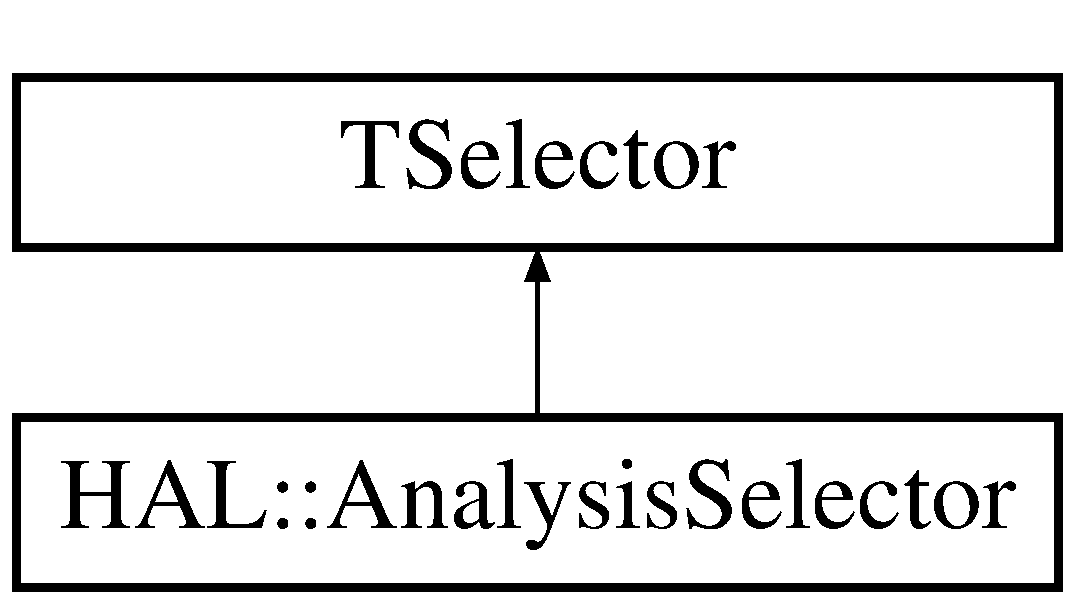
\includegraphics[height=2.000000cm]{class_h_a_l_1_1_analysis_selector}
\end{center}
\end{figure}
\subsection*{Public Member Functions}
\begin{DoxyCompactItemize}
\item 
\hypertarget{class_h_a_l_1_1_analysis_selector_a0e69d567472b846500e3758d0e1cafd3}{{\bfseries Analysis\+Selector} (\hyperlink{class_h_a_l_1_1_algorithm}{Algorithm} $\ast$af, T\+Tree $\ast$=0)}\label{class_h_a_l_1_1_analysis_selector_a0e69d567472b846500e3758d0e1cafd3}

\item 
\hypertarget{class_h_a_l_1_1_analysis_selector_a674eacd53bc6d9b2b82d5769ecf4c965}{virtual Int\+\_\+t {\bfseries Version} () const }\label{class_h_a_l_1_1_analysis_selector_a674eacd53bc6d9b2b82d5769ecf4c965}

\item 
\hypertarget{class_h_a_l_1_1_analysis_selector_aee810e2db449acf3c75cf0c7ed085318}{virtual void {\bfseries Begin} (T\+Tree $\ast$tree)}\label{class_h_a_l_1_1_analysis_selector_aee810e2db449acf3c75cf0c7ed085318}

\item 
\hypertarget{class_h_a_l_1_1_analysis_selector_a47feee7290d251295e65bc69b4e5b982}{virtual void {\bfseries Slave\+Begin} (T\+Tree $\ast$tree)}\label{class_h_a_l_1_1_analysis_selector_a47feee7290d251295e65bc69b4e5b982}

\item 
\hypertarget{class_h_a_l_1_1_analysis_selector_a73f70c38aab67b59e030bfa3e5182d3c}{virtual void {\bfseries Init} (T\+Tree $\ast$tree)}\label{class_h_a_l_1_1_analysis_selector_a73f70c38aab67b59e030bfa3e5182d3c}

\item 
\hypertarget{class_h_a_l_1_1_analysis_selector_a5ce023e4ee2bbc1d6ea0437175258195}{virtual Bool\+\_\+t {\bfseries Notify} ()}\label{class_h_a_l_1_1_analysis_selector_a5ce023e4ee2bbc1d6ea0437175258195}

\item 
\hypertarget{class_h_a_l_1_1_analysis_selector_ad89da1b73776f3acd5e8200d51438e47}{virtual Bool\+\_\+t {\bfseries Process} (Long64\+\_\+t entry)}\label{class_h_a_l_1_1_analysis_selector_ad89da1b73776f3acd5e8200d51438e47}

\item 
\hypertarget{class_h_a_l_1_1_analysis_selector_ae34c9fc9d657cea4c277306043997440}{virtual Int\+\_\+t {\bfseries Get\+Entry} (Long64\+\_\+t entry, Int\+\_\+t getall=0)}\label{class_h_a_l_1_1_analysis_selector_ae34c9fc9d657cea4c277306043997440}

\item 
\hypertarget{class_h_a_l_1_1_analysis_selector_a8e8f2ff599b95b4ea1437080f7a243e2}{virtual void {\bfseries Set\+Option} (const char $\ast$option)}\label{class_h_a_l_1_1_analysis_selector_a8e8f2ff599b95b4ea1437080f7a243e2}

\item 
\hypertarget{class_h_a_l_1_1_analysis_selector_a6c5b330612cbb40740a1773322f1bd4c}{virtual void {\bfseries Set\+Object} (T\+Object $\ast$obj)}\label{class_h_a_l_1_1_analysis_selector_a6c5b330612cbb40740a1773322f1bd4c}

\item 
\hypertarget{class_h_a_l_1_1_analysis_selector_a2ad21fe9c786a8b8ed9d2f2ed03b18dd}{virtual void {\bfseries Set\+Input\+List} (T\+List $\ast$input)}\label{class_h_a_l_1_1_analysis_selector_a2ad21fe9c786a8b8ed9d2f2ed03b18dd}

\item 
\hypertarget{class_h_a_l_1_1_analysis_selector_af839fdbf6d731039f3dfe2a28435cfa0}{virtual T\+List $\ast$ {\bfseries Get\+Output\+List} () const }\label{class_h_a_l_1_1_analysis_selector_af839fdbf6d731039f3dfe2a28435cfa0}

\item 
\hypertarget{class_h_a_l_1_1_analysis_selector_a83767cc68a8016682064a673b4cd3a81}{virtual void {\bfseries Slave\+Terminate} ()}\label{class_h_a_l_1_1_analysis_selector_a83767cc68a8016682064a673b4cd3a81}

\item 
\hypertarget{class_h_a_l_1_1_analysis_selector_a8b660b6a333cdefd12e1829389fbf0cd}{virtual void {\bfseries Terminate} ()}\label{class_h_a_l_1_1_analysis_selector_a8b660b6a333cdefd12e1829389fbf0cd}

\item 
\hypertarget{class_h_a_l_1_1_analysis_selector_a65b63a6f47a198031436edbea7818b1b}{void {\bfseries Set\+Output\+File\+Name} (T\+String fname)}\label{class_h_a_l_1_1_analysis_selector_a65b63a6f47a198031436edbea7818b1b}

\item 
\hypertarget{class_h_a_l_1_1_analysis_selector_a03cb0fb32fb595a20183a10651811a10}{void {\bfseries Set\+Output\+Tree\+Name} (T\+String tname)}\label{class_h_a_l_1_1_analysis_selector_a03cb0fb32fb595a20183a10651811a10}

\item 
\hypertarget{class_h_a_l_1_1_analysis_selector_ab1610526942d045e9bc1b2e4006575a5}{void {\bfseries Set\+Output\+Tree\+Description} (T\+String tdescription)}\label{class_h_a_l_1_1_analysis_selector_ab1610526942d045e9bc1b2e4006575a5}

\item 
\hypertarget{class_h_a_l_1_1_analysis_selector_a1e12ce6668b8f66ee0590dab7d9a6904}{void {\bfseries Set\+Message\+Period} (unsigned p=0)}\label{class_h_a_l_1_1_analysis_selector_a1e12ce6668b8f66ee0590dab7d9a6904}

\end{DoxyCompactItemize}
\subsection*{Public Attributes}
\begin{DoxyCompactItemize}
\item 
\hypertarget{class_h_a_l_1_1_analysis_selector_a7634b6d0eb916c352968a1a6acd7f3d2}{\hyperlink{class_h_a_l_1_1_algorithm}{Algorithm} $\ast$ {\bfseries f\+Analysis\+Flow}}\label{class_h_a_l_1_1_analysis_selector_a7634b6d0eb916c352968a1a6acd7f3d2}

\item 
\hypertarget{class_h_a_l_1_1_analysis_selector_a37f6980439f0b1e94db036220eacef8f}{T\+Tree $\ast$ {\bfseries f\+Chain}}\label{class_h_a_l_1_1_analysis_selector_a37f6980439f0b1e94db036220eacef8f}

\item 
\hypertarget{class_h_a_l_1_1_analysis_selector_a4d6e0e029b502012c4bf6d4f1618625c}{T\+Map $\ast$ \hyperlink{class_h_a_l_1_1_analysis_selector_a4d6e0e029b502012c4bf6d4f1618625c}{f\+Branch\+Map}}\label{class_h_a_l_1_1_analysis_selector_a4d6e0e029b502012c4bf6d4f1618625c}

\begin{DoxyCompactList}\small\item\em pointer to the analyzed T\+Tree or T\+Chain \end{DoxyCompactList}\end{DoxyCompactItemize}


The documentation for this class was generated from the following file\+:\begin{DoxyCompactItemize}
\item 
/\+Users/jhetherly/src/\+H\+A\+L-\/\+R\+O\+O\+T/include/\+H\+A\+L/Analysis\+Selector.\+h\end{DoxyCompactItemize}

\hypertarget{class_h_a_l_1_1_analysis_tree_reader}{\section{H\+A\+L\+:\+:Analysis\+Tree\+Reader Class Reference}
\label{class_h_a_l_1_1_analysis_tree_reader}\index{H\+A\+L\+::\+Analysis\+Tree\+Reader@{H\+A\+L\+::\+Analysis\+Tree\+Reader}}
}


Class for the easy extraction of data from a T\+Tree.  




{\ttfamily \#include $<$Analysis\+Tree\+Reader.\+h$>$}

Inheritance diagram for H\+A\+L\+:\+:Analysis\+Tree\+Reader\+:\begin{figure}[H]
\begin{center}
\leavevmode
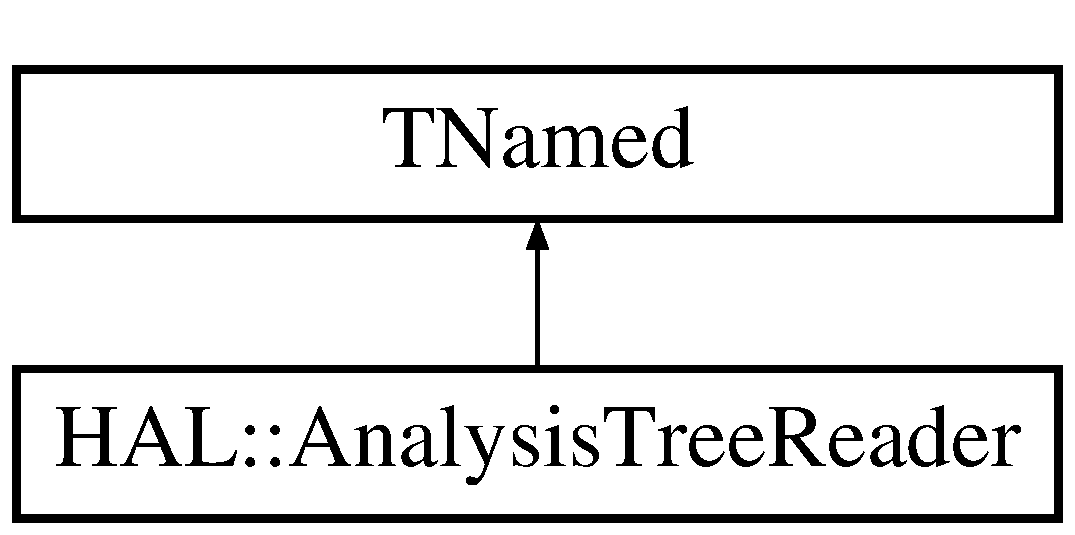
\includegraphics[height=2.000000cm]{class_h_a_l_1_1_analysis_tree_reader}
\end{center}
\end{figure}
\subsection*{Public Member Functions}
\begin{DoxyCompactItemize}
\item 
\hypertarget{class_h_a_l_1_1_analysis_tree_reader_ac00ba35d0b860566482e32c1dfd04827}{{\bfseries Analysis\+Tree\+Reader} (T\+Tree $\ast$tree=0)}\label{class_h_a_l_1_1_analysis_tree_reader_ac00ba35d0b860566482e32c1dfd04827}

\item 
\hypertarget{class_h_a_l_1_1_analysis_tree_reader_a031181c782d3620d271a92cef995d998}{void {\bfseries Set\+Tree} (T\+Tree $\ast$tree)}\label{class_h_a_l_1_1_analysis_tree_reader_a031181c782d3620d271a92cef995d998}

\item 
\hypertarget{class_h_a_l_1_1_analysis_tree_reader_a1a9c8bc30141df5fab1163f006fb08e3}{void {\bfseries Set\+Entry} (Long64\+\_\+t entry)}\label{class_h_a_l_1_1_analysis_tree_reader_a1a9c8bc30141df5fab1163f006fb08e3}

\item 
\hypertarget{class_h_a_l_1_1_analysis_tree_reader_a6fcf94a452ec53b66d9e0e49062d4e44}{Long64\+\_\+t {\bfseries Get\+Entry\+Number} ()}\label{class_h_a_l_1_1_analysis_tree_reader_a6fcf94a452ec53b66d9e0e49062d4e44}

\item 
\hypertarget{class_h_a_l_1_1_analysis_tree_reader_a6ad8933bd6c8cc2b17179c96fd3bfcb1}{T\+Tree $\ast$ {\bfseries Get\+Tree} ()}\label{class_h_a_l_1_1_analysis_tree_reader_a6ad8933bd6c8cc2b17179c96fd3bfcb1}

\item 
\hypertarget{class_h_a_l_1_1_analysis_tree_reader_a85f301e0ef78fdf1f239b36a030fb023}{T\+String {\bfseries Get\+Branch\+Name} (const T\+String \&name)}\label{class_h_a_l_1_1_analysis_tree_reader_a85f301e0ef78fdf1f239b36a030fb023}

\item 
\hypertarget{class_h_a_l_1_1_analysis_tree_reader_ab17ea6c10da56d9282d60d9507e01ef9}{void {\bfseries Init} ()}\label{class_h_a_l_1_1_analysis_tree_reader_ab17ea6c10da56d9282d60d9507e01ef9}

\item 
\hypertarget{class_h_a_l_1_1_analysis_tree_reader_adfe7aa4110b150fb1c7e80580a775a82}{Bool\+\_\+t {\bfseries Notify} ()}\label{class_h_a_l_1_1_analysis_tree_reader_adfe7aa4110b150fb1c7e80580a775a82}

\item 
\hypertarget{class_h_a_l_1_1_analysis_tree_reader_ae3dcc57b2cc27431e89edd341b300eb6}{void {\bfseries Set\+Branch\+Map} (T\+Map $\ast$m)}\label{class_h_a_l_1_1_analysis_tree_reader_ae3dcc57b2cc27431e89edd341b300eb6}

\item 
\hypertarget{class_h_a_l_1_1_analysis_tree_reader_afa371719adcfa583fe29ea0f468b9ea8}{bool {\bfseries Check\+Branch\+Map\+Nickname} (const T\+String \&name)}\label{class_h_a_l_1_1_analysis_tree_reader_afa371719adcfa583fe29ea0f468b9ea8}

\item 
\hypertarget{class_h_a_l_1_1_analysis_tree_reader_aa4dae5db1c660155760ded68007cdd6d}{unsigned int {\bfseries Get\+Rank} (const T\+String \&branchname)}\label{class_h_a_l_1_1_analysis_tree_reader_aa4dae5db1c660155760ded68007cdd6d}

\item 
\hypertarget{class_h_a_l_1_1_analysis_tree_reader_a1a8c741c6b2ae788b98d596c12543724}{unsigned int {\bfseries Get\+Dim} (const T\+String \&branchname, const long long \&idx\+\_\+1=-\/1)}\label{class_h_a_l_1_1_analysis_tree_reader_a1a8c741c6b2ae788b98d596c12543724}

\item 
\hypertarget{class_h_a_l_1_1_analysis_tree_reader_a8a76466f4746d4764b0fa97416182267}{bool {\bfseries Get\+Bool} (const T\+String \&branchname, const long long \&idx\+\_\+1=-\/1, const long long \&idx\+\_\+2=-\/1)}\label{class_h_a_l_1_1_analysis_tree_reader_a8a76466f4746d4764b0fa97416182267}

\item 
\hypertarget{class_h_a_l_1_1_analysis_tree_reader_a6b2e01f1075ed295513a268258d3d559}{long long {\bfseries Get\+Integer} (const T\+String \&branchname, const long long \&idx\+\_\+1=-\/1, const long long \&idx\+\_\+2=-\/1)}\label{class_h_a_l_1_1_analysis_tree_reader_a6b2e01f1075ed295513a268258d3d559}

\item 
\hypertarget{class_h_a_l_1_1_analysis_tree_reader_aa4d264484021ba0912f6254aeacc784f}{unsigned long long {\bfseries Get\+Counting} (const T\+String \&branchname, const long long \&idx\+\_\+1=-\/1, const long long \&idx\+\_\+2=-\/1)}\label{class_h_a_l_1_1_analysis_tree_reader_aa4d264484021ba0912f6254aeacc784f}

\item 
\hypertarget{class_h_a_l_1_1_analysis_tree_reader_a4a3dd2065768228ab817575307c4691e}{long double {\bfseries Get\+Decimal} (const T\+String \&branchname, const long long \&idx\+\_\+1=-\/1, const long long \&idx\+\_\+2=-\/1)}\label{class_h_a_l_1_1_analysis_tree_reader_a4a3dd2065768228ab817575307c4691e}

\item 
\hypertarget{class_h_a_l_1_1_analysis_tree_reader_a75c0fe7d907ac8f1792ff496e4cf0b73}{T\+String {\bfseries Get\+String} (const T\+String \&branchname, const long long \&idx\+\_\+1=-\/1, const long long \&idx\+\_\+2=-\/1)}\label{class_h_a_l_1_1_analysis_tree_reader_a75c0fe7d907ac8f1792ff496e4cf0b73}

\item 
\hypertarget{class_h_a_l_1_1_analysis_tree_reader_ad44870dd8478b8d404ede307726f2db6}{T\+Obj\+Array \& {\bfseries Get\+Obj\+Array} (const T\+String \&branchname, const long long \&idx\+\_\+1=-\/1)}\label{class_h_a_l_1_1_analysis_tree_reader_ad44870dd8478b8d404ede307726f2db6}

\item 
\hypertarget{class_h_a_l_1_1_analysis_tree_reader_ae9115ce6bba555009b6b21eca20339c9}{T\+Clones\+Array \& {\bfseries Get\+Clones\+Array} (const T\+String \&branchname, const long long \&idx\+\_\+1=-\/1)}\label{class_h_a_l_1_1_analysis_tree_reader_ae9115ce6bba555009b6b21eca20339c9}

\item 
\hypertarget{class_h_a_l_1_1_analysis_tree_reader_af010b9fafb8bd7f06efcaa46d1360253}{T\+Ref \& {\bfseries Get\+Ref} (const T\+String \&branchname, const long long \&idx\+\_\+1=-\/1, const long long \&idx\+\_\+2=-\/1)}\label{class_h_a_l_1_1_analysis_tree_reader_af010b9fafb8bd7f06efcaa46d1360253}

\item 
\hypertarget{class_h_a_l_1_1_analysis_tree_reader_a66bc43933f69938b94dd8caf5277395c}{T\+Ref\+Array \& {\bfseries Get\+Ref\+Array} (const T\+String \&branchname, const long long \&idx\+\_\+1=-\/1)}\label{class_h_a_l_1_1_analysis_tree_reader_a66bc43933f69938b94dd8caf5277395c}

\item 
\hypertarget{class_h_a_l_1_1_analysis_tree_reader_ad8be72de7b7f4ae5ced82c636ac91dd1}{{\bfseries Class\+Def} (\hyperlink{class_h_a_l_1_1_analysis_tree_reader}{Analysis\+Tree\+Reader}, 0)}\label{class_h_a_l_1_1_analysis_tree_reader_ad8be72de7b7f4ae5ced82c636ac91dd1}

\end{DoxyCompactItemize}
\subsection*{Friends}
\begin{DoxyCompactItemize}
\item 
\hypertarget{class_h_a_l_1_1_analysis_tree_reader_a3da00472573022c08436f19e0a48d8de}{class {\bfseries internal\+::\+Branch\+Manager}}\label{class_h_a_l_1_1_analysis_tree_reader_a3da00472573022c08436f19e0a48d8de}

\end{DoxyCompactItemize}


\subsection{Detailed Description}
Class for the easy extraction of data from a T\+Tree. 

This class allows for the easy retrieval of data stored in a T\+Tree. Through normal function calls the user can access data stored as scalars, C-\/arrays, S\+T\+L vectors, 2\+D C-\/arrays, and S\+T\+L vectors of vectors. A listing of the allowable types is given below. If a class that is stored in the T\+Tree can be decomposed in 'Make\+Class\+Mode,' this class can read it as well. The user should not need to worry about allocating memory or setting branch addresses. There are hard limits to the lengths of a C-\/array and 2\+D C-\/array that can be read. They are 10000 and 10000x100 respectively. If \hyperlink{namespace_h_a_l}{H\+A\+L} is compiled with R\+O\+O\+T version 6 or later, this restriction is lifted.~\newline
{\itshape Data Types That Can be Read\+:} \begin{TabularC}{6}
\hline
\rowcolor{lightgray}\PBS\centering {\bf Boolean }&\PBS\centering {\bf Integer }&\PBS\centering {\bf Counting }&\PBS\centering {\bf Decimal }&\PBS\centering {\bf String }&\PBS\centering {\bf Misc  }\\\cline{1-6}
\PBS\centering bool/\+Bool\+\_\+t &\PBS\centering int/\+Int\+\_\+t &\PBS\centering unsigned int/\+U\+Int\+\_\+t &\PBS\centering float/\+Float\+\_\+t/\+Float16\+\_\+t/\+Real\+\_\+t &\PBS\centering char/\+Char\+\_\+t/\+Text\+\_\+t &\PBS\centering T\+Obj\+Array \\\cline{1-6}
\PBS\centering &\PBS\centering short/\+Short\+\_\+t &\PBS\centering unsigned short/\+U\+Short\+\_\+t &\PBS\centering double/\+Double\+\_\+t/\+Double32\+\_\+t &\PBS\centering char$\ast$ &\PBS\centering T\+Clones\+Array \\\cline{1-6}
\PBS\centering &\PBS\centering long/\+Long\+\_\+t &\PBS\centering unsigned long/\+U\+Long\+\_\+t &\PBS\centering long double/\+Long\+Double\+\_\+t &\PBS\centering T\+String &\PBS\centering T\+Ref \\\cline{1-6}
\PBS\centering &\PBS\centering long long/\+Long64\+\_\+t &\PBS\centering unsigned long long/\+U\+Long64\+\_\+t &\PBS\centering &\PBS\centering T\+Obj\+String &\PBS\centering T\+Ref\+Array \\\cline{1-6}
\PBS\centering &\PBS\centering signed char &\PBS\centering unsigned char &\PBS\centering &\PBS\centering std\+::string &\PBS\centering T\+Ref\+Array \\\cline{1-6}
\end{TabularC}


The documentation for this class was generated from the following file\+:\begin{DoxyCompactItemize}
\item 
/\+Users/jhetherly/src/\+H\+A\+L-\/\+R\+O\+O\+T/include/\+H\+A\+L/\hyperlink{_analysis_tree_reader_8h}{Analysis\+Tree\+Reader.\+h}\end{DoxyCompactItemize}

\hypertarget{class_h_a_l_1_1_analysis_tree_writer}{\section{H\-A\-L\-:\-:Analysis\-Tree\-Writer Class Reference}
\label{class_h_a_l_1_1_analysis_tree_writer}\index{H\-A\-L\-::\-Analysis\-Tree\-Writer@{H\-A\-L\-::\-Analysis\-Tree\-Writer}}
}
Inheritance diagram for H\-A\-L\-:\-:Analysis\-Tree\-Writer\-:\begin{figure}[H]
\begin{center}
\leavevmode
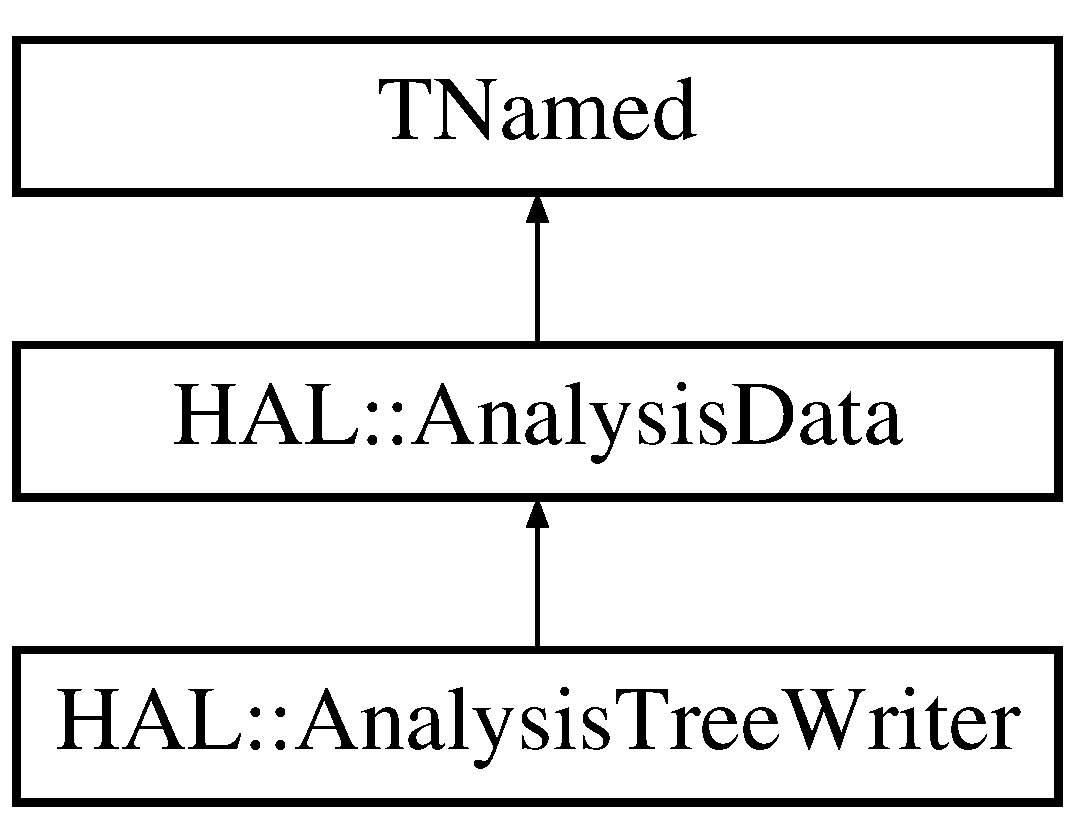
\includegraphics[height=3.000000cm]{class_h_a_l_1_1_analysis_tree_writer}
\end{center}
\end{figure}
\subsection*{Public Member Functions}
\begin{DoxyCompactItemize}
\item 
\hypertarget{class_h_a_l_1_1_analysis_tree_writer_a84bd5498078ffc6e67d5265b907705d5}{{\bfseries Analysis\-Tree\-Writer} (const T\-String \&ofile)}\label{class_h_a_l_1_1_analysis_tree_writer_a84bd5498078ffc6e67d5265b907705d5}

\item 
\hypertarget{class_h_a_l_1_1_analysis_tree_writer_a54d51c4078ebaeedd2ce02ac73945a78}{void {\bfseries Set\-Tree\-Name} (const T\-String \&tname)}\label{class_h_a_l_1_1_analysis_tree_writer_a54d51c4078ebaeedd2ce02ac73945a78}

\item 
\hypertarget{class_h_a_l_1_1_analysis_tree_writer_aec457c9a3f813a0ed455e1e4933ddb7f}{void {\bfseries Set\-Tree\-Description} (const T\-String \&tdescription)}\label{class_h_a_l_1_1_analysis_tree_writer_aec457c9a3f813a0ed455e1e4933ddb7f}

\item 
\hypertarget{class_h_a_l_1_1_analysis_tree_writer_a7e27d118b04eeba4c7fe66185c07434b}{void {\bfseries Set\-Tree\-For\-Branch} (const T\-String \&tree, const T\-String \&branch)}\label{class_h_a_l_1_1_analysis_tree_writer_a7e27d118b04eeba4c7fe66185c07434b}

\item 
\hypertarget{class_h_a_l_1_1_analysis_tree_writer_a91582d11e58a4b8d84d4ff35123a3ad3}{T\-String {\bfseries Get\-Tree\-For\-Branch} (const T\-String \&branch)}\label{class_h_a_l_1_1_analysis_tree_writer_a91582d11e58a4b8d84d4ff35123a3ad3}

\item 
\hypertarget{class_h_a_l_1_1_analysis_tree_writer_a2bc77354335ee48351205af7804356fc}{void {\bfseries Increment\-Count} ()}\label{class_h_a_l_1_1_analysis_tree_writer_a2bc77354335ee48351205af7804356fc}

\item 
\hypertarget{class_h_a_l_1_1_analysis_tree_writer_af49d85d3524d21a7da1a27d0a029239d}{void {\bfseries Write\-Data} ()}\label{class_h_a_l_1_1_analysis_tree_writer_af49d85d3524d21a7da1a27d0a029239d}

\item 
\hypertarget{class_h_a_l_1_1_analysis_tree_writer_af8dfdc6182004a8931d9c0f8926ae330}{virtual void {\bfseries Set\-Value} (const T\-String \&n, const bool \&v)}\label{class_h_a_l_1_1_analysis_tree_writer_af8dfdc6182004a8931d9c0f8926ae330}

\item 
\hypertarget{class_h_a_l_1_1_analysis_tree_writer_a85b8b7790bb9392ed1d865daab3248d7}{virtual void {\bfseries Set\-Value} (const T\-String \&n, const bool \&v, const long long \&i)}\label{class_h_a_l_1_1_analysis_tree_writer_a85b8b7790bb9392ed1d865daab3248d7}

\item 
\hypertarget{class_h_a_l_1_1_analysis_tree_writer_a2e68fdea10ca87aebab5332c2b680286}{virtual void {\bfseries Set\-Value} (const T\-String \&n, const long double \&v)}\label{class_h_a_l_1_1_analysis_tree_writer_a2e68fdea10ca87aebab5332c2b680286}

\item 
\hypertarget{class_h_a_l_1_1_analysis_tree_writer_ae4fbd939b2edfc2c3859ca24f635a475}{virtual void {\bfseries Set\-Value} (const T\-String \&n, const long double \&v, const long long \&i)}\label{class_h_a_l_1_1_analysis_tree_writer_ae4fbd939b2edfc2c3859ca24f635a475}

\item 
\hypertarget{class_h_a_l_1_1_analysis_tree_writer_a73bed978557c7222f4c88b71c1b74424}{virtual void {\bfseries Set\-Value} (const T\-String \&n, const long long \&v)}\label{class_h_a_l_1_1_analysis_tree_writer_a73bed978557c7222f4c88b71c1b74424}

\item 
\hypertarget{class_h_a_l_1_1_analysis_tree_writer_abc1b0d49980dfe48e99cf3c03f271bb3}{virtual void {\bfseries Set\-Value} (const T\-String \&n, const long long \&v, const long long \&i)}\label{class_h_a_l_1_1_analysis_tree_writer_abc1b0d49980dfe48e99cf3c03f271bb3}

\item 
\hypertarget{class_h_a_l_1_1_analysis_tree_writer_ad7fc39378d544f275cbb19145def8fbf}{virtual void {\bfseries Set\-Value} (const T\-String \&n, const unsigned long long \&v)}\label{class_h_a_l_1_1_analysis_tree_writer_ad7fc39378d544f275cbb19145def8fbf}

\item 
\hypertarget{class_h_a_l_1_1_analysis_tree_writer_ae71437812731ea60b3375c771ff912e1}{virtual void {\bfseries Set\-Value} (const T\-String \&n, const unsigned long long \&v, const long long \&i)}\label{class_h_a_l_1_1_analysis_tree_writer_ae71437812731ea60b3375c771ff912e1}

\item 
\hypertarget{class_h_a_l_1_1_analysis_tree_writer_a77da0342b01b89846c418b825d3a9d99}{{\bfseries Class\-Def\-N\-V} (\hyperlink{class_h_a_l_1_1_analysis_tree_writer}{Analysis\-Tree\-Writer}, 0)}\label{class_h_a_l_1_1_analysis_tree_writer_a77da0342b01b89846c418b825d3a9d99}

\end{DoxyCompactItemize}
\subsection*{Additional Inherited Members}


The documentation for this class was generated from the following file\-:\begin{DoxyCompactItemize}
\item 
/\-Users/jhetherly/src/root\-\_\-\-H\-A\-L/include/\-H\-A\-L/Analysis\-Tree\-Writer.\-h\end{DoxyCompactItemize}

\hypertarget{class_h_a_l_1_1_cut_algorithm}{\section{H\+A\+L\+:\+:Cut\+Algorithm Class Reference}
\label{class_h_a_l_1_1_cut_algorithm}\index{H\+A\+L\+::\+Cut\+Algorithm@{H\+A\+L\+::\+Cut\+Algorithm}}
}
Inheritance diagram for H\+A\+L\+:\+:Cut\+Algorithm\+:\begin{figure}[H]
\begin{center}
\leavevmode
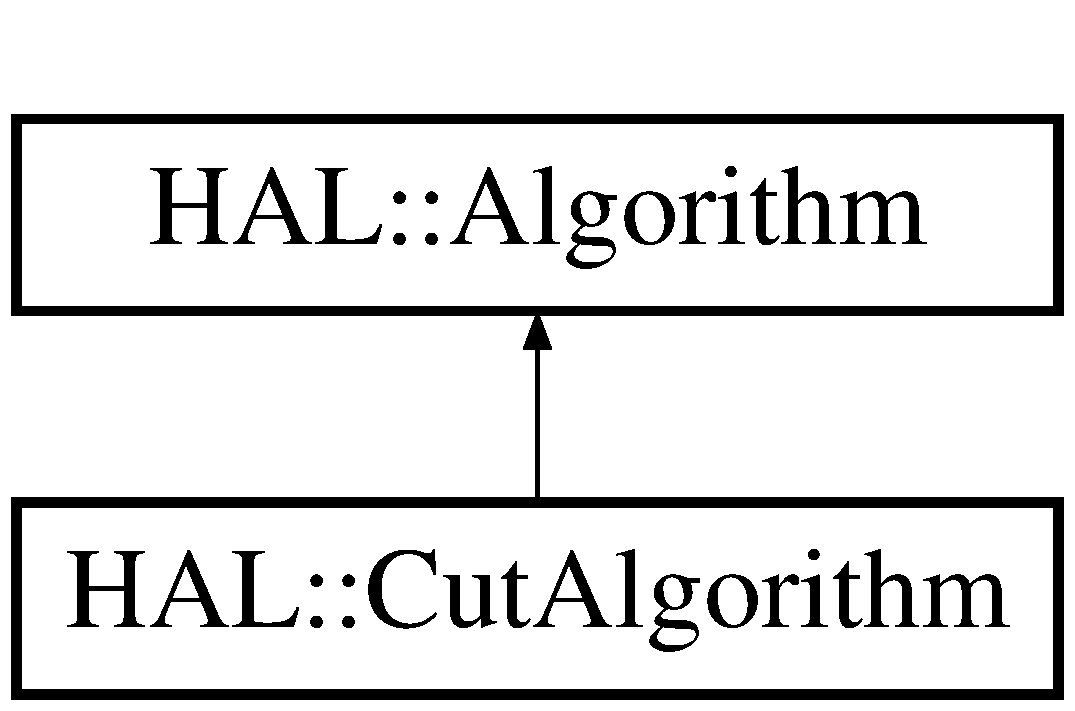
\includegraphics[height=3.000000cm]{class_h_a_l_1_1_cut_algorithm}
\end{center}
\end{figure}
\subsection*{Public Member Functions}
\begin{DoxyCompactItemize}
\item 
\hypertarget{class_h_a_l_1_1_cut_algorithm_a7009161a2b8463fddb9d6336cb2ef669}{{\bfseries Cut\+Algorithm} (T\+String name=\char`\"{}\char`\"{}, T\+String title=\char`\"{}\char`\"{})}\label{class_h_a_l_1_1_cut_algorithm_a7009161a2b8463fddb9d6336cb2ef669}

\end{DoxyCompactItemize}
\subsection*{Protected Member Functions}
\begin{DoxyCompactItemize}
\item 
\hypertarget{class_h_a_l_1_1_cut_algorithm_ad41a2ea5664562c3331f85bcc85317be}{void {\bfseries Passed} ()}\label{class_h_a_l_1_1_cut_algorithm_ad41a2ea5664562c3331f85bcc85317be}

\end{DoxyCompactItemize}
\subsection*{Additional Inherited Members}


The documentation for this class was generated from the following file\+:\begin{DoxyCompactItemize}
\item 
/\+Users/jhetherly/src/\+H\+A\+L-\/\+R\+O\+O\+T/include/\+H\+A\+L/Cut\+Algorithm.\+h\end{DoxyCompactItemize}

\hypertarget{class_h_a_l_1_1_cut_optimizer}{\section{H\+A\+L\+:\+:Cut\+Optimizer Class Reference}
\label{class_h_a_l_1_1_cut_optimizer}\index{H\+A\+L\+::\+Cut\+Optimizer@{H\+A\+L\+::\+Cut\+Optimizer}}
}
\subsection*{Public Member Functions}
\begin{DoxyCompactItemize}
\item 
\hypertarget{class_h_a_l_1_1_cut_optimizer_a7f1be065a4ec07a1e8cfee59dc0b80d1}{{\bfseries Cut\+Optimizer} (T\+F2 $\ast$st=N\+U\+L\+L)}\label{class_h_a_l_1_1_cut_optimizer_a7f1be065a4ec07a1e8cfee59dc0b80d1}

\item 
\hypertarget{class_h_a_l_1_1_cut_optimizer_a89082c3ec2719462ba90b3677119a1c6}{void {\bfseries Set\+Fitness\+Function} (T\+F2 $\ast$st=N\+U\+L\+L)}\label{class_h_a_l_1_1_cut_optimizer_a89082c3ec2719462ba90b3677119a1c6}

\item 
\hypertarget{class_h_a_l_1_1_cut_optimizer_a35eab754a13b06da0526fdf9900cc6eb}{T\+F2 $\ast$ {\bfseries Get\+Fitness\+Function} ()}\label{class_h_a_l_1_1_cut_optimizer_a35eab754a13b06da0526fdf9900cc6eb}

\item 
\hypertarget{class_h_a_l_1_1_cut_optimizer_a7055834b45ab96cbe30d335f7cd6f26d}{T\+Matrix\+D $\ast$ {\bfseries Optimize} (T\+H1 $\ast$sig, T\+H1 $\ast$bkg, Int\+\_\+t n, T\+String side=\char`\"{}both\char`\"{}, Int\+\_\+t rebin=1, Double\+\_\+t x\+\_\+min=T\+Math\+::\+Quiet\+Na\+N(), Double\+\_\+t x\+\_\+max=T\+Math\+::\+Quiet\+Na\+N())}\label{class_h_a_l_1_1_cut_optimizer_a7055834b45ab96cbe30d335f7cd6f26d}

\end{DoxyCompactItemize}


The documentation for this class was generated from the following file\+:\begin{DoxyCompactItemize}
\item 
/\+Users/jhetherly/src/\+H\+A\+L-\/\+R\+O\+O\+T/include/\+H\+A\+L/Cut\+Optimizer.\+h\end{DoxyCompactItemize}

\hypertarget{class_h_a_l_1_1_f_a0000}{\section{H\-A\-L\-:\-:F\-A0000 Class Reference}
\label{class_h_a_l_1_1_f_a0000}\index{H\-A\-L\-::\-F\-A0000@{H\-A\-L\-::\-F\-A0000}}
}
Inheritance diagram for H\-A\-L\-:\-:F\-A0000\-:\begin{figure}[H]
\begin{center}
\leavevmode
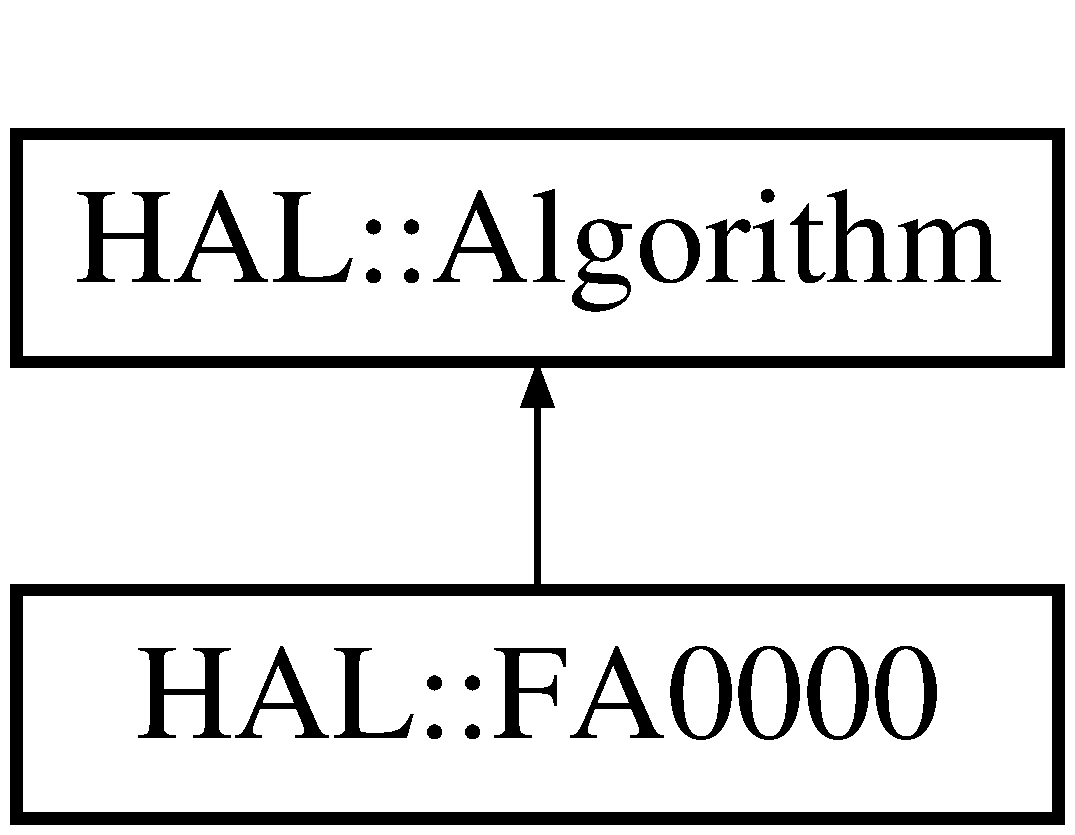
\includegraphics[height=2.000000cm]{class_h_a_l_1_1_f_a0000}
\end{center}
\end{figure}
\subsection*{Public Member Functions}
\begin{DoxyCompactItemize}
\item 
\hypertarget{class_h_a_l_1_1_f_a0000_aad6722776f282a5c7c371bd3537301a7}{{\bfseries F\-A0000} (T\-String name, T\-String title, T\-String input, unsigned n)}\label{class_h_a_l_1_1_f_a0000_aad6722776f282a5c7c371bd3537301a7}

\end{DoxyCompactItemize}
\subsection*{Protected Member Functions}
\begin{DoxyCompactItemize}
\item 
\hypertarget{class_h_a_l_1_1_f_a0000_a4c52d10b435893775de1226d13f4e4a3}{virtual void {\bfseries Exec} (Option\-\_\-t $\ast$)}\label{class_h_a_l_1_1_f_a0000_a4c52d10b435893775de1226d13f4e4a3}

\end{DoxyCompactItemize}
\subsection*{Additional Inherited Members}


The documentation for this class was generated from the following file\-:\begin{DoxyCompactItemize}
\item 
/\-Users/jhetherly/src/root\-\_\-\-H\-A\-L/include/\-H\-A\-L/Algorithms.\-h\end{DoxyCompactItemize}

\hypertarget{class_h_a_l_1_1_h_a_l_exception}{\section{H\+A\+L\+:\+:H\+A\+L\+Exception Class Reference}
\label{class_h_a_l_1_1_h_a_l_exception}\index{H\+A\+L\+::\+H\+A\+L\+Exception@{H\+A\+L\+::\+H\+A\+L\+Exception}}
}
Inheritance diagram for H\+A\+L\+:\+:H\+A\+L\+Exception\+:\begin{figure}[H]
\begin{center}
\leavevmode
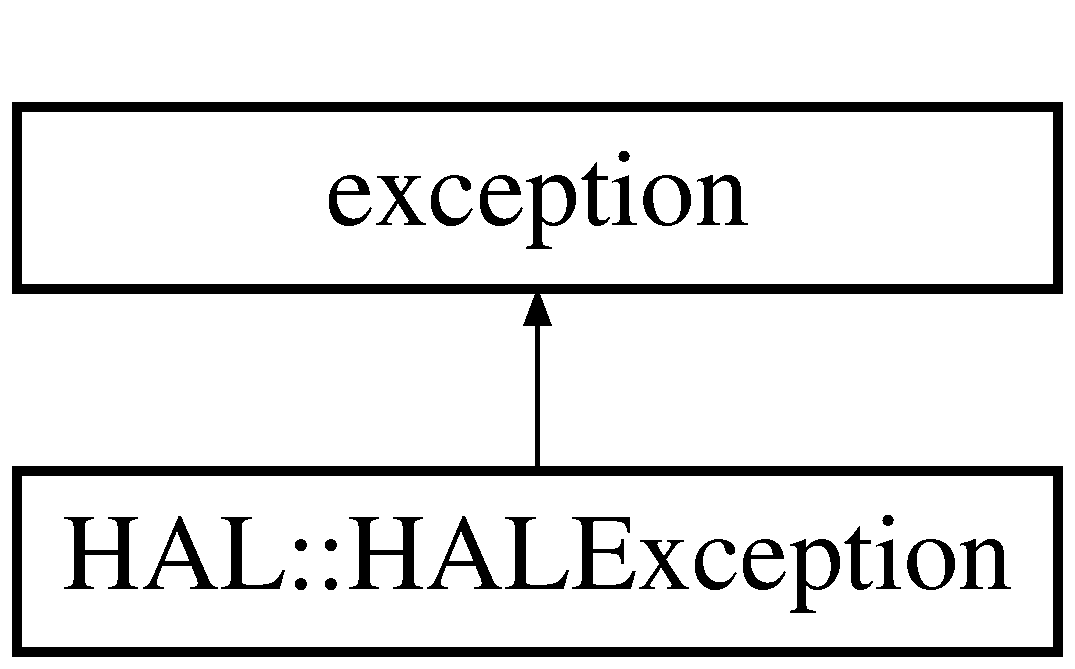
\includegraphics[height=2.000000cm]{class_h_a_l_1_1_h_a_l_exception}
\end{center}
\end{figure}
\subsection*{Public Member Functions}
\begin{DoxyCompactItemize}
\item 
\hypertarget{class_h_a_l_1_1_h_a_l_exception_a4f6662db7819d278a642abc8edf6b064}{{\bfseries H\+A\+L\+Exception} (T\+String m)}\label{class_h_a_l_1_1_h_a_l_exception_a4f6662db7819d278a642abc8edf6b064}

\item 
\hypertarget{class_h_a_l_1_1_h_a_l_exception_aaf6b8a29e7bb09721dd7aaa7b7a9b078}{virtual const char $\ast$ {\bfseries what} () const   throw ()}\label{class_h_a_l_1_1_h_a_l_exception_aaf6b8a29e7bb09721dd7aaa7b7a9b078}

\end{DoxyCompactItemize}


The documentation for this class was generated from the following file\+:\begin{DoxyCompactItemize}
\item 
/\+Users/jhetherly/src/\+H\+A\+L-\/\+R\+O\+O\+T/include/\+H\+A\+L/Exceptions.\+h\end{DoxyCompactItemize}

\hypertarget{class_h_a_l_1_1_i_a0000}{\section{H\-A\-L\-:\-:I\-A0000 Class Reference}
\label{class_h_a_l_1_1_i_a0000}\index{H\-A\-L\-::\-I\-A0000@{H\-A\-L\-::\-I\-A0000}}
}
Inheritance diagram for H\-A\-L\-:\-:I\-A0000\-:\begin{figure}[H]
\begin{center}
\leavevmode
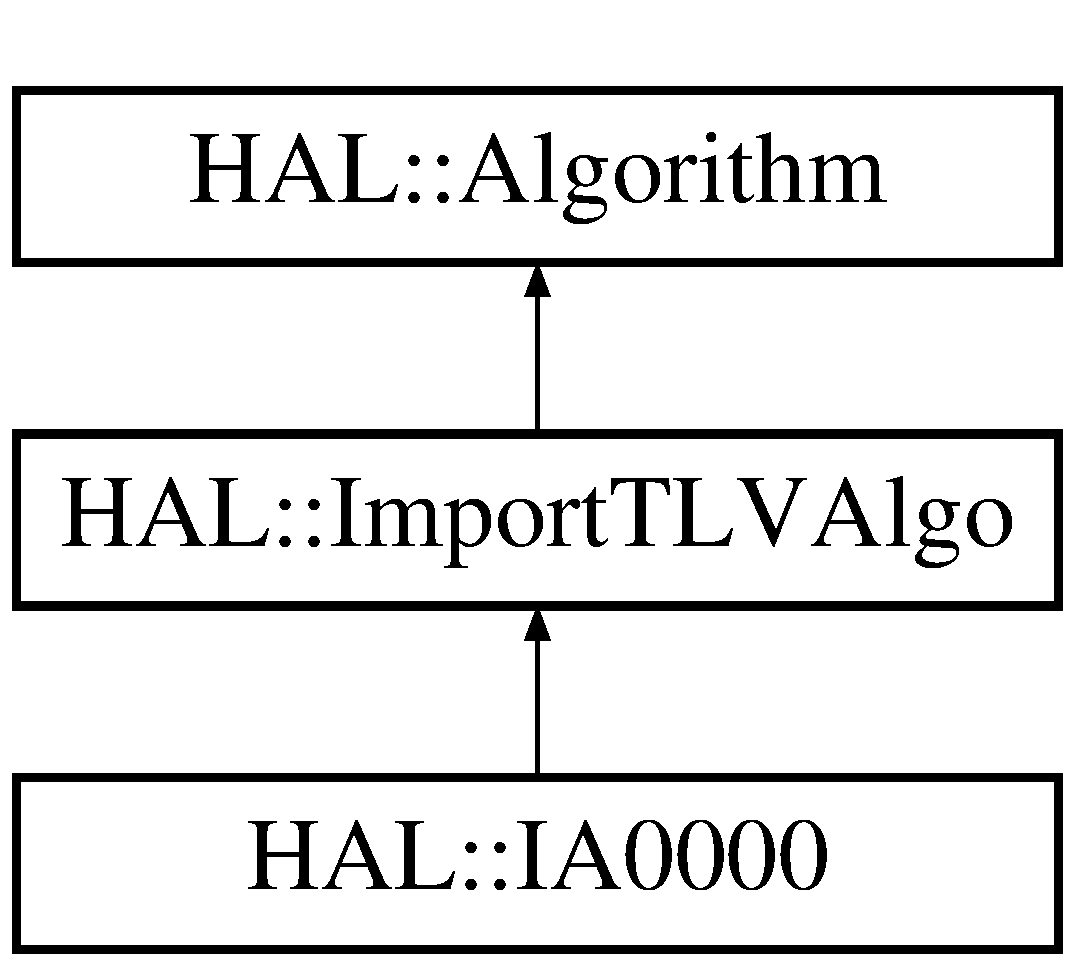
\includegraphics[height=3.000000cm]{class_h_a_l_1_1_i_a0000}
\end{center}
\end{figure}
\subsection*{Public Member Functions}
\begin{DoxyCompactItemize}
\item 
\hypertarget{class_h_a_l_1_1_i_a0000_a50a9cf30836e759d26cf2e3cb3084749}{{\bfseries I\-A0000} (T\-String name, T\-String title)}\label{class_h_a_l_1_1_i_a0000_a50a9cf30836e759d26cf2e3cb3084749}

\end{DoxyCompactItemize}
\subsection*{Protected Member Functions}
\begin{DoxyCompactItemize}
\item 
\hypertarget{class_h_a_l_1_1_i_a0000_a1c2bfacb12fd984648c5bf91ca2a4e79}{virtual void {\bfseries Exec} (Option\-\_\-t $\ast$)}\label{class_h_a_l_1_1_i_a0000_a1c2bfacb12fd984648c5bf91ca2a4e79}

\item 
\hypertarget{class_h_a_l_1_1_i_a0000_aacf10223fa251dc1655ac7bafb5599b2}{virtual T\-Lorentz\-Vector $\ast$ {\bfseries Make\-T\-L\-V} (unsigned)}\label{class_h_a_l_1_1_i_a0000_aacf10223fa251dc1655ac7bafb5599b2}

\end{DoxyCompactItemize}
\subsection*{Additional Inherited Members}


The documentation for this class was generated from the following file\-:\begin{DoxyCompactItemize}
\item 
/\-Users/jhetherly/src/root\-\_\-\-H\-A\-L/include/\-H\-A\-L/Algorithms.\-h\end{DoxyCompactItemize}

\hypertarget{class_h_a_l_1_1_i_a0001}{\section{H\-A\-L\-:\-:I\-A0001 Class Reference}
\label{class_h_a_l_1_1_i_a0001}\index{H\-A\-L\-::\-I\-A0001@{H\-A\-L\-::\-I\-A0001}}
}
Inheritance diagram for H\-A\-L\-:\-:I\-A0001\-:\begin{figure}[H]
\begin{center}
\leavevmode
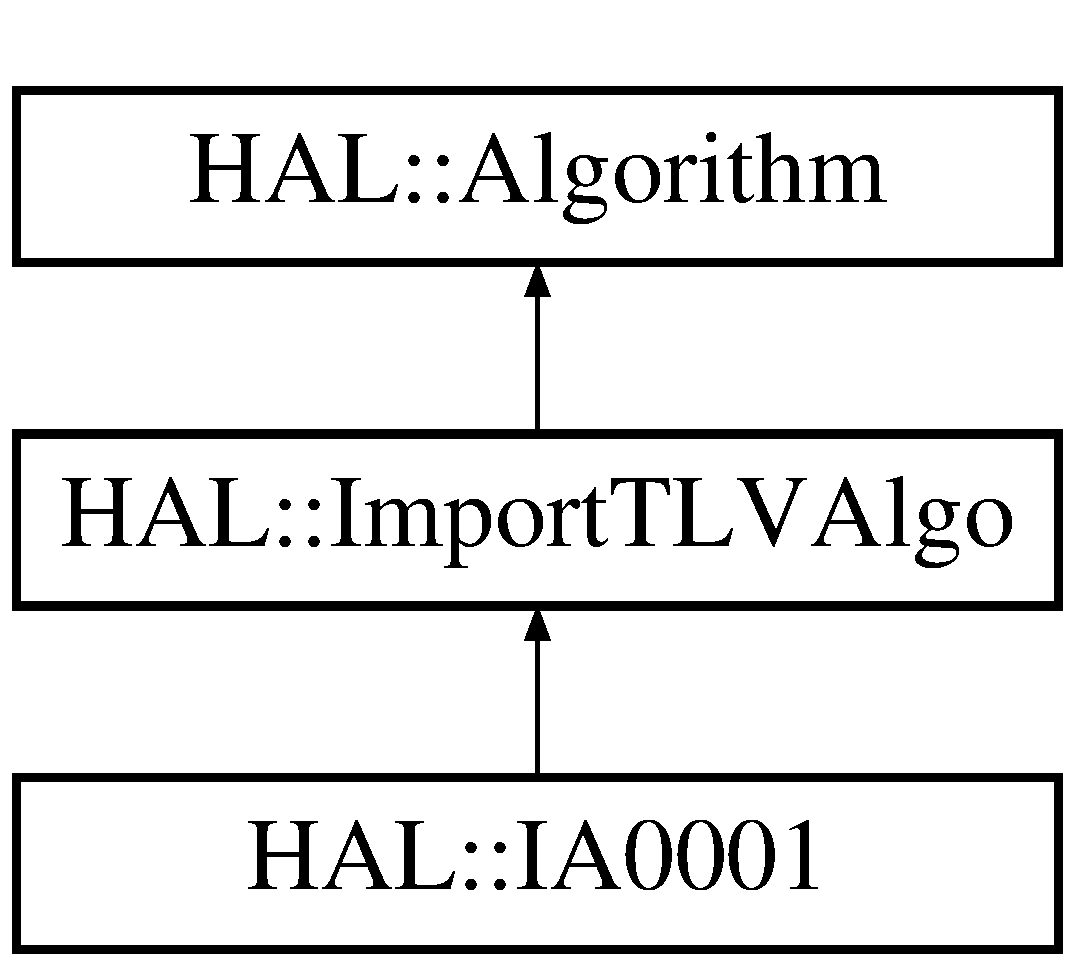
\includegraphics[height=3.000000cm]{class_h_a_l_1_1_i_a0001}
\end{center}
\end{figure}
\subsection*{Public Member Functions}
\begin{DoxyCompactItemize}
\item 
\hypertarget{class_h_a_l_1_1_i_a0001_a297e0a7b26f6b0cf7669d15c4492cde9}{{\bfseries I\-A0001} (T\-String name, T\-String title)}\label{class_h_a_l_1_1_i_a0001_a297e0a7b26f6b0cf7669d15c4492cde9}

\end{DoxyCompactItemize}
\subsection*{Protected Member Functions}
\begin{DoxyCompactItemize}
\item 
\hypertarget{class_h_a_l_1_1_i_a0001_a5e66185dd1be784cc1e619fcb3350f6b}{virtual void {\bfseries Exec} (Option\-\_\-t $\ast$)}\label{class_h_a_l_1_1_i_a0001_a5e66185dd1be784cc1e619fcb3350f6b}

\item 
\hypertarget{class_h_a_l_1_1_i_a0001_a4e97323778e70612eae8978afdb6243f}{virtual T\-Lorentz\-Vector $\ast$ {\bfseries Make\-T\-L\-V} (unsigned)}\label{class_h_a_l_1_1_i_a0001_a4e97323778e70612eae8978afdb6243f}

\end{DoxyCompactItemize}
\subsection*{Additional Inherited Members}


The documentation for this class was generated from the following file\-:\begin{DoxyCompactItemize}
\item 
/\-Users/jhetherly/src/root\-\_\-\-H\-A\-L/include/\-H\-A\-L/Algorithms.\-h\end{DoxyCompactItemize}

\hypertarget{class_h_a_l_1_1_i_a0002}{\section{H\-A\-L\-:\-:I\-A0002 Class Reference}
\label{class_h_a_l_1_1_i_a0002}\index{H\-A\-L\-::\-I\-A0002@{H\-A\-L\-::\-I\-A0002}}
}
Inheritance diagram for H\-A\-L\-:\-:I\-A0002\-:\begin{figure}[H]
\begin{center}
\leavevmode
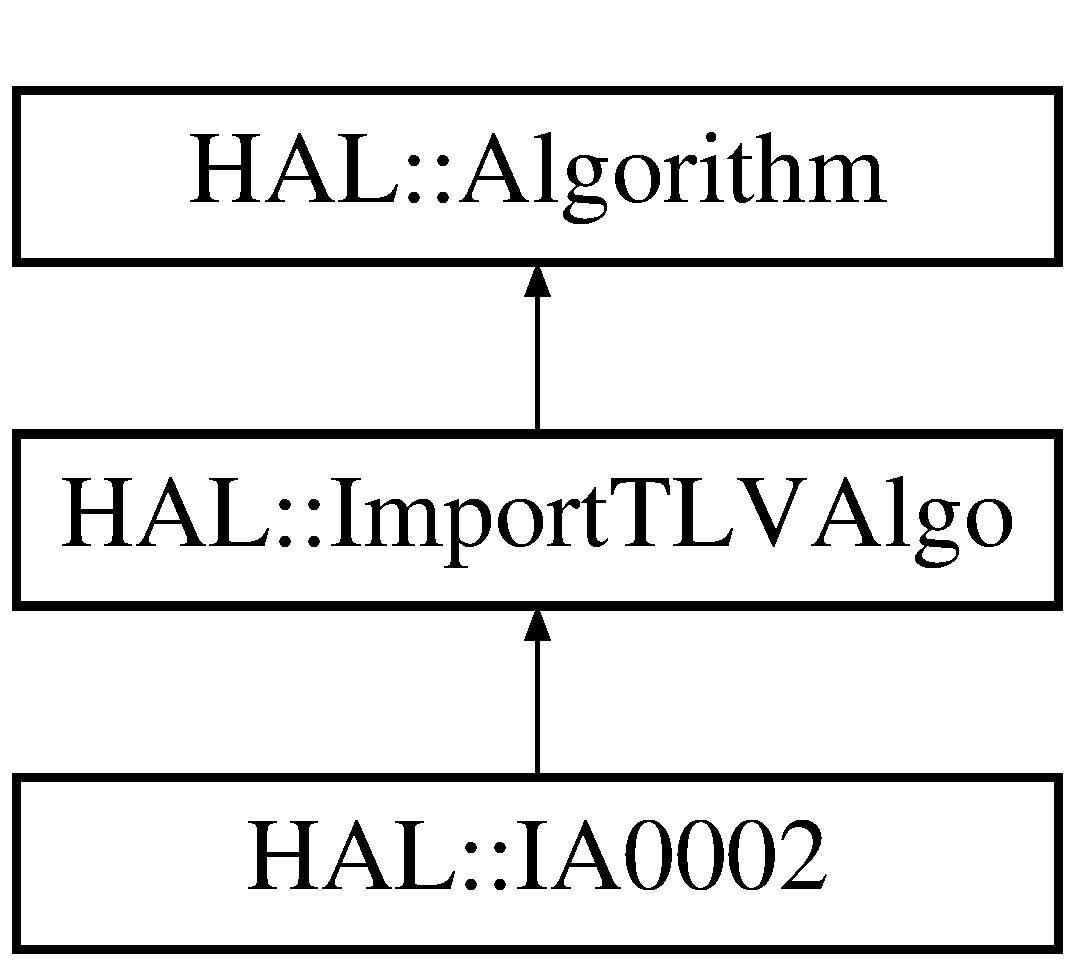
\includegraphics[height=3.000000cm]{class_h_a_l_1_1_i_a0002}
\end{center}
\end{figure}
\subsection*{Public Member Functions}
\begin{DoxyCompactItemize}
\item 
\hypertarget{class_h_a_l_1_1_i_a0002_a81c04000d15411704c132cb249c2c382}{{\bfseries I\-A0002} (T\-String name, T\-String title, unsigned n)}\label{class_h_a_l_1_1_i_a0002_a81c04000d15411704c132cb249c2c382}

\end{DoxyCompactItemize}
\subsection*{Protected Member Functions}
\begin{DoxyCompactItemize}
\item 
\hypertarget{class_h_a_l_1_1_i_a0002_a364552f858102f8dce07701cc665101f}{virtual void {\bfseries Exec} (Option\-\_\-t $\ast$)}\label{class_h_a_l_1_1_i_a0002_a364552f858102f8dce07701cc665101f}

\item 
\hypertarget{class_h_a_l_1_1_i_a0002_a2b602a3be3bc043b8d8b5423f759361b}{virtual T\-Lorentz\-Vector $\ast$ {\bfseries Make\-T\-L\-V} (unsigned)}\label{class_h_a_l_1_1_i_a0002_a2b602a3be3bc043b8d8b5423f759361b}

\end{DoxyCompactItemize}
\subsection*{Additional Inherited Members}


The documentation for this class was generated from the following file\-:\begin{DoxyCompactItemize}
\item 
/\-Users/jhetherly/src/root\-\_\-\-H\-A\-L/include/\-H\-A\-L/Algorithms.\-h\end{DoxyCompactItemize}

\hypertarget{class_h_a_l_1_1_i_a0010}{\section{H\-A\-L\-:\-:I\-A0010 Class Reference}
\label{class_h_a_l_1_1_i_a0010}\index{H\-A\-L\-::\-I\-A0010@{H\-A\-L\-::\-I\-A0010}}
}
Inheritance diagram for H\-A\-L\-:\-:I\-A0010\-:\begin{figure}[H]
\begin{center}
\leavevmode
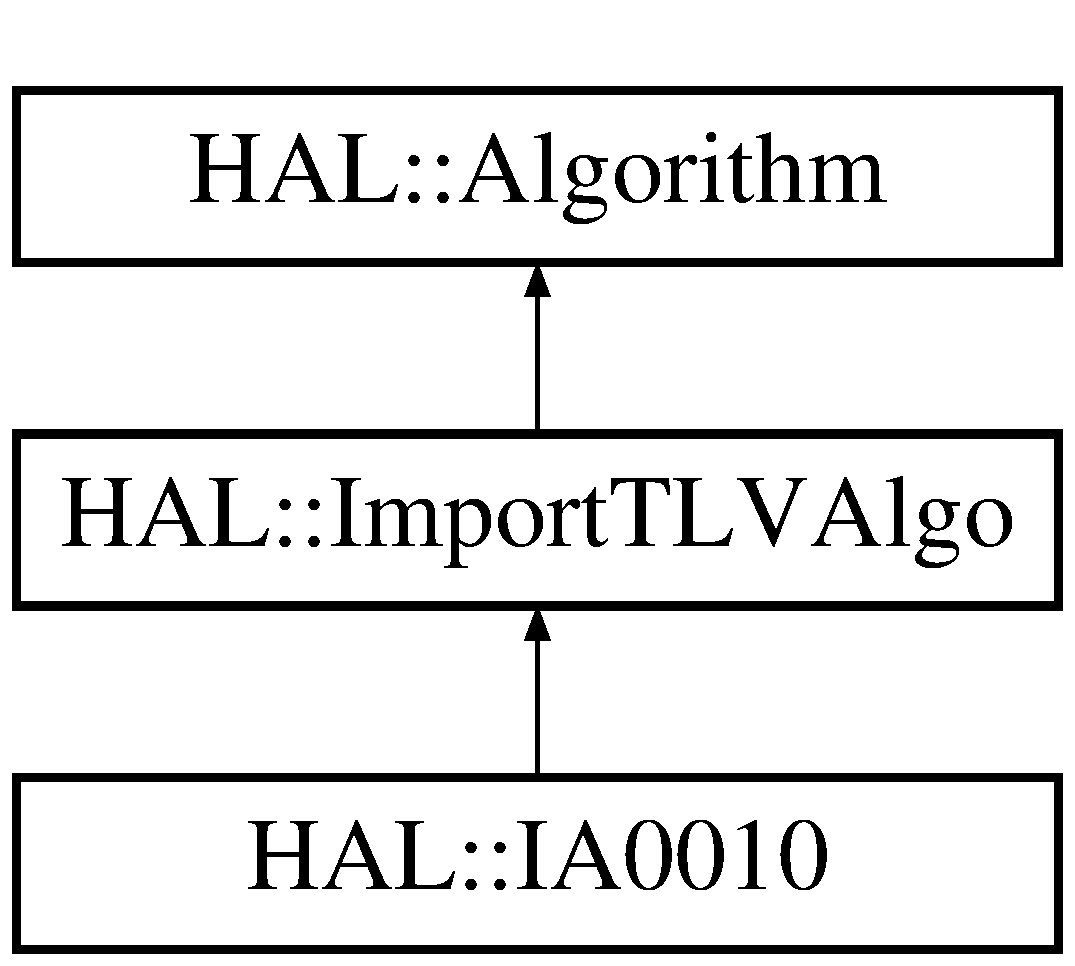
\includegraphics[height=3.000000cm]{class_h_a_l_1_1_i_a0010}
\end{center}
\end{figure}
\subsection*{Public Member Functions}
\begin{DoxyCompactItemize}
\item 
\hypertarget{class_h_a_l_1_1_i_a0010_a019328281bbe7934bda23775b45cbe1a}{{\bfseries I\-A0010} (T\-String name, T\-String title)}\label{class_h_a_l_1_1_i_a0010_a019328281bbe7934bda23775b45cbe1a}

\end{DoxyCompactItemize}
\subsection*{Protected Member Functions}
\begin{DoxyCompactItemize}
\item 
\hypertarget{class_h_a_l_1_1_i_a0010_aeb97ff037be8078385f303643ae0b5f7}{virtual void {\bfseries Exec} (Option\-\_\-t $\ast$)}\label{class_h_a_l_1_1_i_a0010_aeb97ff037be8078385f303643ae0b5f7}

\item 
\hypertarget{class_h_a_l_1_1_i_a0010_a2bf414a4ed29feb050fcffb6d093057e}{virtual T\-Lorentz\-Vector $\ast$ {\bfseries Make\-T\-L\-V} (unsigned)}\label{class_h_a_l_1_1_i_a0010_a2bf414a4ed29feb050fcffb6d093057e}

\end{DoxyCompactItemize}
\subsection*{Additional Inherited Members}


The documentation for this class was generated from the following file\-:\begin{DoxyCompactItemize}
\item 
/\-Users/jhetherly/src/root\-\_\-\-H\-A\-L/include/\-H\-A\-L/Algorithms.\-h\end{DoxyCompactItemize}

\hypertarget{class_h_a_l_1_1_i_a0011}{\section{H\-A\-L\-:\-:I\-A0011 Class Reference}
\label{class_h_a_l_1_1_i_a0011}\index{H\-A\-L\-::\-I\-A0011@{H\-A\-L\-::\-I\-A0011}}
}
Inheritance diagram for H\-A\-L\-:\-:I\-A0011\-:\begin{figure}[H]
\begin{center}
\leavevmode
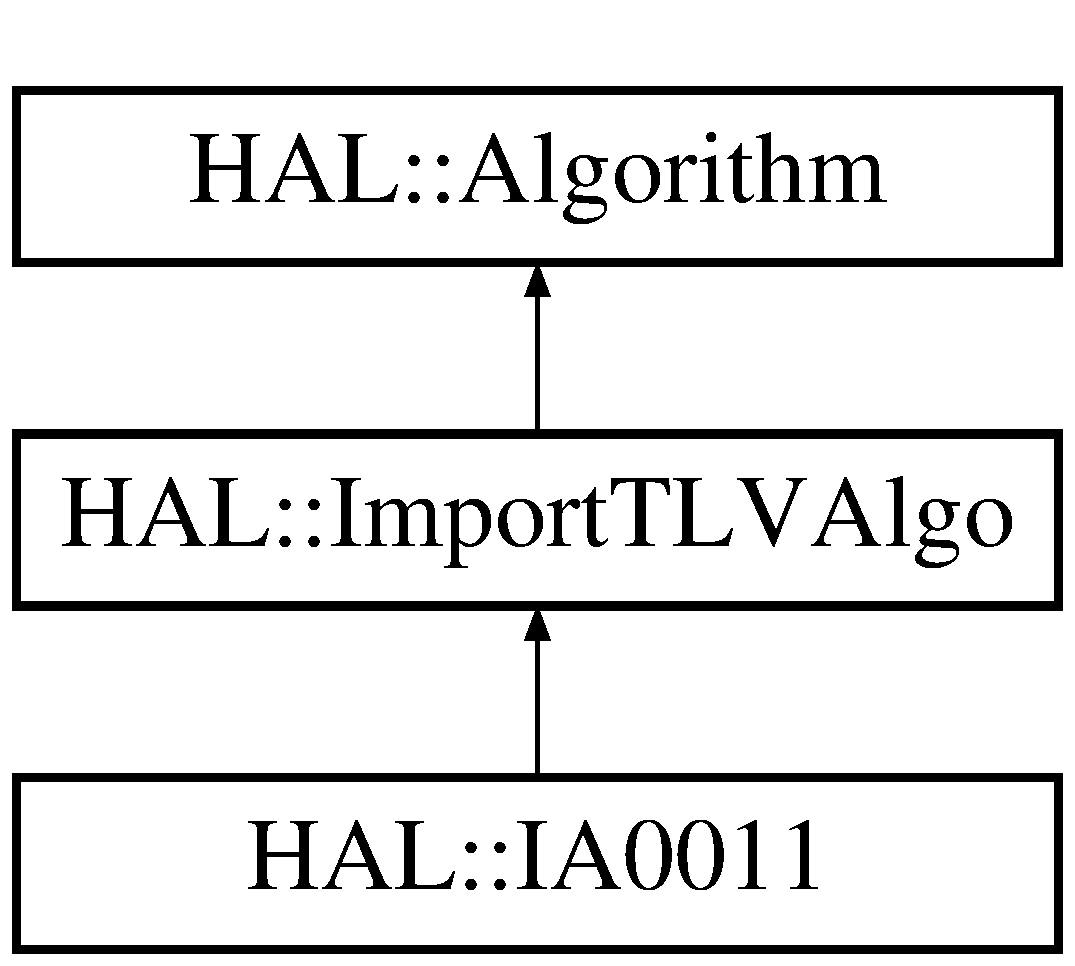
\includegraphics[height=3.000000cm]{class_h_a_l_1_1_i_a0011}
\end{center}
\end{figure}
\subsection*{Public Member Functions}
\begin{DoxyCompactItemize}
\item 
\hypertarget{class_h_a_l_1_1_i_a0011_a97e917fb60b60941fcb9cbea062ef4f3}{{\bfseries I\-A0011} (T\-String name, T\-String title)}\label{class_h_a_l_1_1_i_a0011_a97e917fb60b60941fcb9cbea062ef4f3}

\end{DoxyCompactItemize}
\subsection*{Protected Member Functions}
\begin{DoxyCompactItemize}
\item 
\hypertarget{class_h_a_l_1_1_i_a0011_a1e098f2695b7ec272206c86366154460}{virtual void {\bfseries Exec} (Option\-\_\-t $\ast$)}\label{class_h_a_l_1_1_i_a0011_a1e098f2695b7ec272206c86366154460}

\item 
\hypertarget{class_h_a_l_1_1_i_a0011_a01ad5ada48b556d3b10e648f6b9687a6}{virtual T\-Lorentz\-Vector $\ast$ {\bfseries Make\-T\-L\-V} (unsigned)}\label{class_h_a_l_1_1_i_a0011_a01ad5ada48b556d3b10e648f6b9687a6}

\end{DoxyCompactItemize}
\subsection*{Additional Inherited Members}


The documentation for this class was generated from the following file\-:\begin{DoxyCompactItemize}
\item 
/\-Users/jhetherly/src/root\-\_\-\-H\-A\-L/include/\-H\-A\-L/Algorithms.\-h\end{DoxyCompactItemize}

\hypertarget{class_h_a_l_1_1_i_a0012}{\section{H\-A\-L\-:\-:I\-A0012 Class Reference}
\label{class_h_a_l_1_1_i_a0012}\index{H\-A\-L\-::\-I\-A0012@{H\-A\-L\-::\-I\-A0012}}
}
Inheritance diagram for H\-A\-L\-:\-:I\-A0012\-:\begin{figure}[H]
\begin{center}
\leavevmode
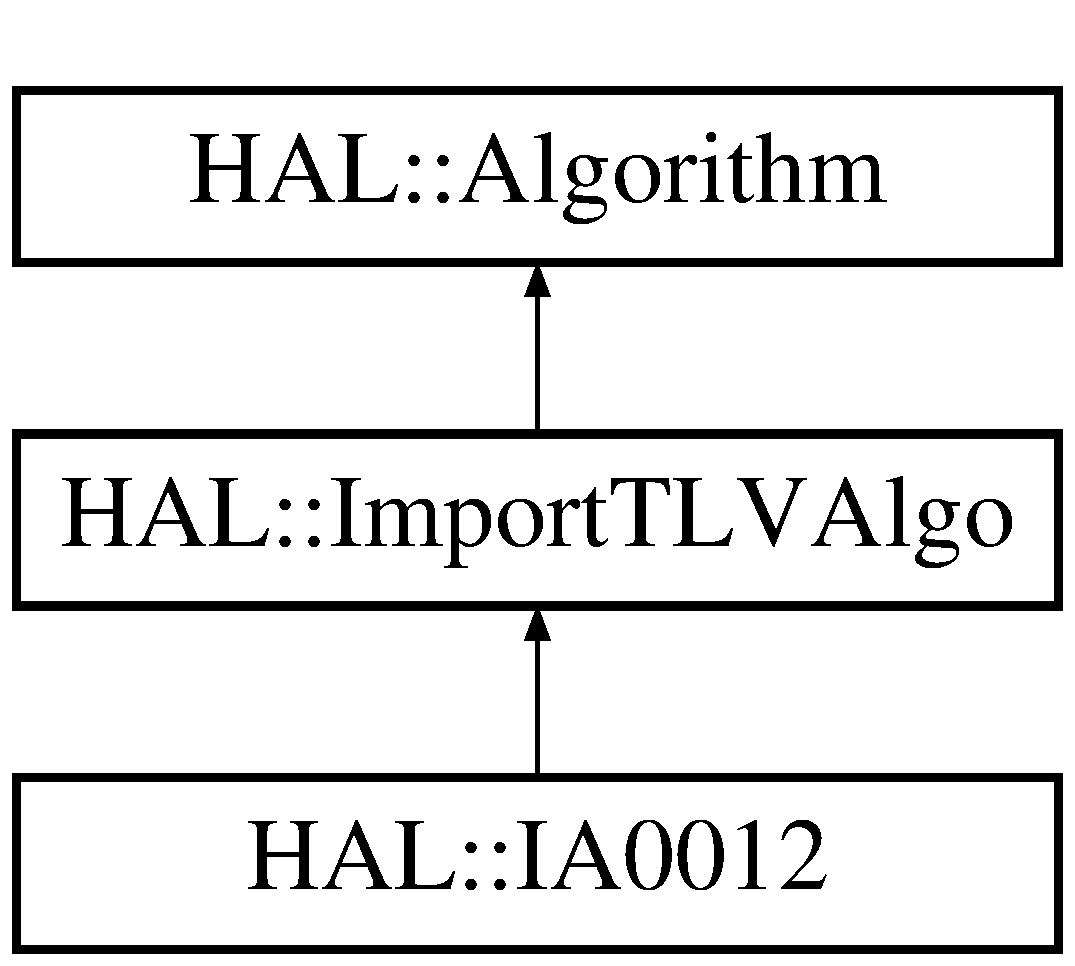
\includegraphics[height=3.000000cm]{class_h_a_l_1_1_i_a0012}
\end{center}
\end{figure}
\subsection*{Public Member Functions}
\begin{DoxyCompactItemize}
\item 
\hypertarget{class_h_a_l_1_1_i_a0012_ab22ce5f648311cc495f8430984edab3f}{{\bfseries I\-A0012} (T\-String name, T\-String title, unsigned n)}\label{class_h_a_l_1_1_i_a0012_ab22ce5f648311cc495f8430984edab3f}

\end{DoxyCompactItemize}
\subsection*{Protected Member Functions}
\begin{DoxyCompactItemize}
\item 
\hypertarget{class_h_a_l_1_1_i_a0012_a94f7cb9185c6f2740357f4ae322dcb0a}{virtual void {\bfseries Exec} (Option\-\_\-t $\ast$)}\label{class_h_a_l_1_1_i_a0012_a94f7cb9185c6f2740357f4ae322dcb0a}

\item 
\hypertarget{class_h_a_l_1_1_i_a0012_aa5014a116be85bc72b2ab11a08a65f3b}{virtual T\-Lorentz\-Vector $\ast$ {\bfseries Make\-T\-L\-V} (unsigned)}\label{class_h_a_l_1_1_i_a0012_aa5014a116be85bc72b2ab11a08a65f3b}

\end{DoxyCompactItemize}
\subsection*{Additional Inherited Members}


The documentation for this class was generated from the following file\-:\begin{DoxyCompactItemize}
\item 
/\-Users/jhetherly/src/root\-\_\-\-H\-A\-L/include/\-H\-A\-L/Algorithms.\-h\end{DoxyCompactItemize}

\hypertarget{class_h_a_l_1_1_i_a0020}{\section{H\-A\-L\-:\-:I\-A0020 Class Reference}
\label{class_h_a_l_1_1_i_a0020}\index{H\-A\-L\-::\-I\-A0020@{H\-A\-L\-::\-I\-A0020}}
}
Inheritance diagram for H\-A\-L\-:\-:I\-A0020\-:\begin{figure}[H]
\begin{center}
\leavevmode
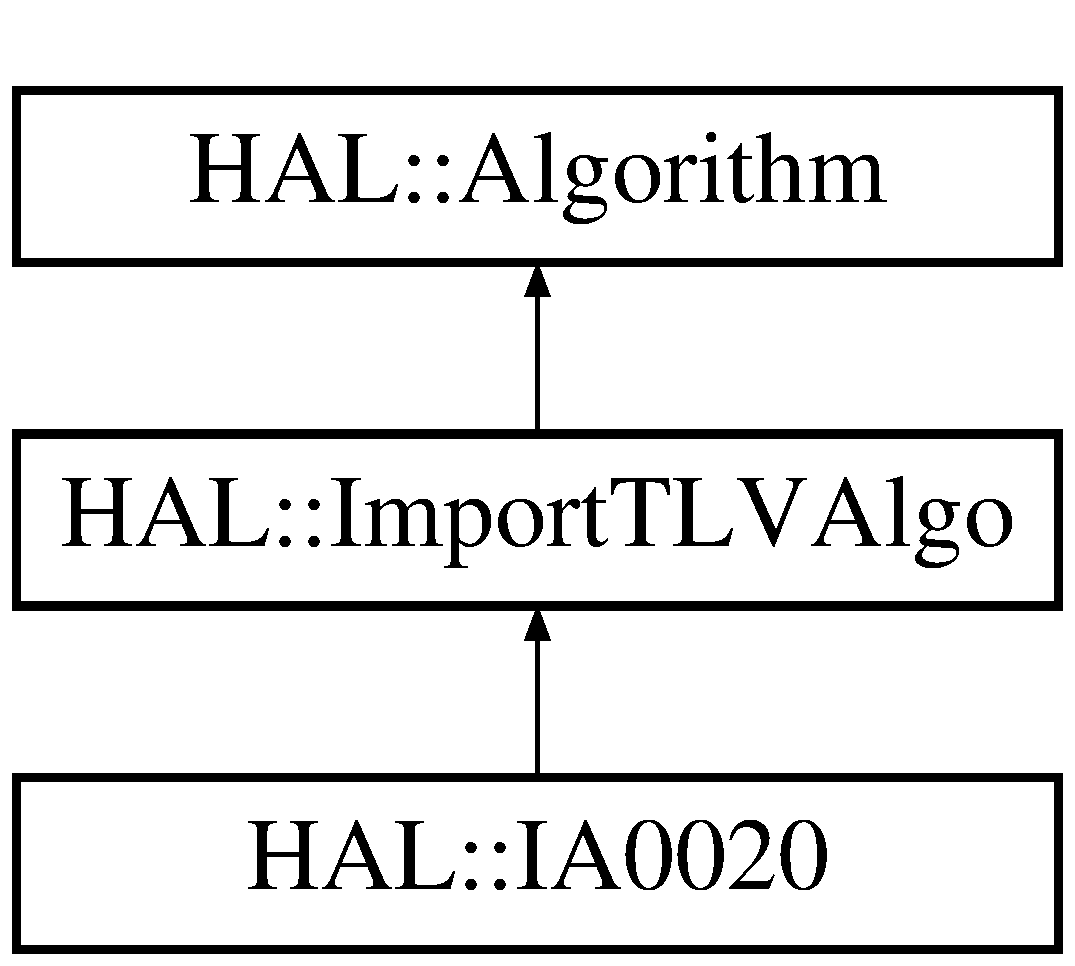
\includegraphics[height=3.000000cm]{class_h_a_l_1_1_i_a0020}
\end{center}
\end{figure}
\subsection*{Public Member Functions}
\begin{DoxyCompactItemize}
\item 
\hypertarget{class_h_a_l_1_1_i_a0020_a7e28d08e71591d8e156164039cb7c07a}{{\bfseries I\-A0020} (T\-String name, T\-String title)}\label{class_h_a_l_1_1_i_a0020_a7e28d08e71591d8e156164039cb7c07a}

\end{DoxyCompactItemize}
\subsection*{Protected Member Functions}
\begin{DoxyCompactItemize}
\item 
\hypertarget{class_h_a_l_1_1_i_a0020_ac2616410fe28dc70d7b6f6883fe8813e}{virtual void {\bfseries Exec} (Option\-\_\-t $\ast$)}\label{class_h_a_l_1_1_i_a0020_ac2616410fe28dc70d7b6f6883fe8813e}

\item 
\hypertarget{class_h_a_l_1_1_i_a0020_aa2b81352888484e42bfc14070c0c9142}{virtual T\-Lorentz\-Vector $\ast$ {\bfseries Make\-T\-L\-V} (unsigned)}\label{class_h_a_l_1_1_i_a0020_aa2b81352888484e42bfc14070c0c9142}

\end{DoxyCompactItemize}
\subsection*{Additional Inherited Members}


The documentation for this class was generated from the following file\-:\begin{DoxyCompactItemize}
\item 
/\-Users/jhetherly/src/root\-\_\-\-H\-A\-L/include/\-H\-A\-L/Algorithms.\-h\end{DoxyCompactItemize}

\hypertarget{class_h_a_l_1_1_i_a0021}{\section{H\-A\-L\-:\-:I\-A0021 Class Reference}
\label{class_h_a_l_1_1_i_a0021}\index{H\-A\-L\-::\-I\-A0021@{H\-A\-L\-::\-I\-A0021}}
}
Inheritance diagram for H\-A\-L\-:\-:I\-A0021\-:\begin{figure}[H]
\begin{center}
\leavevmode
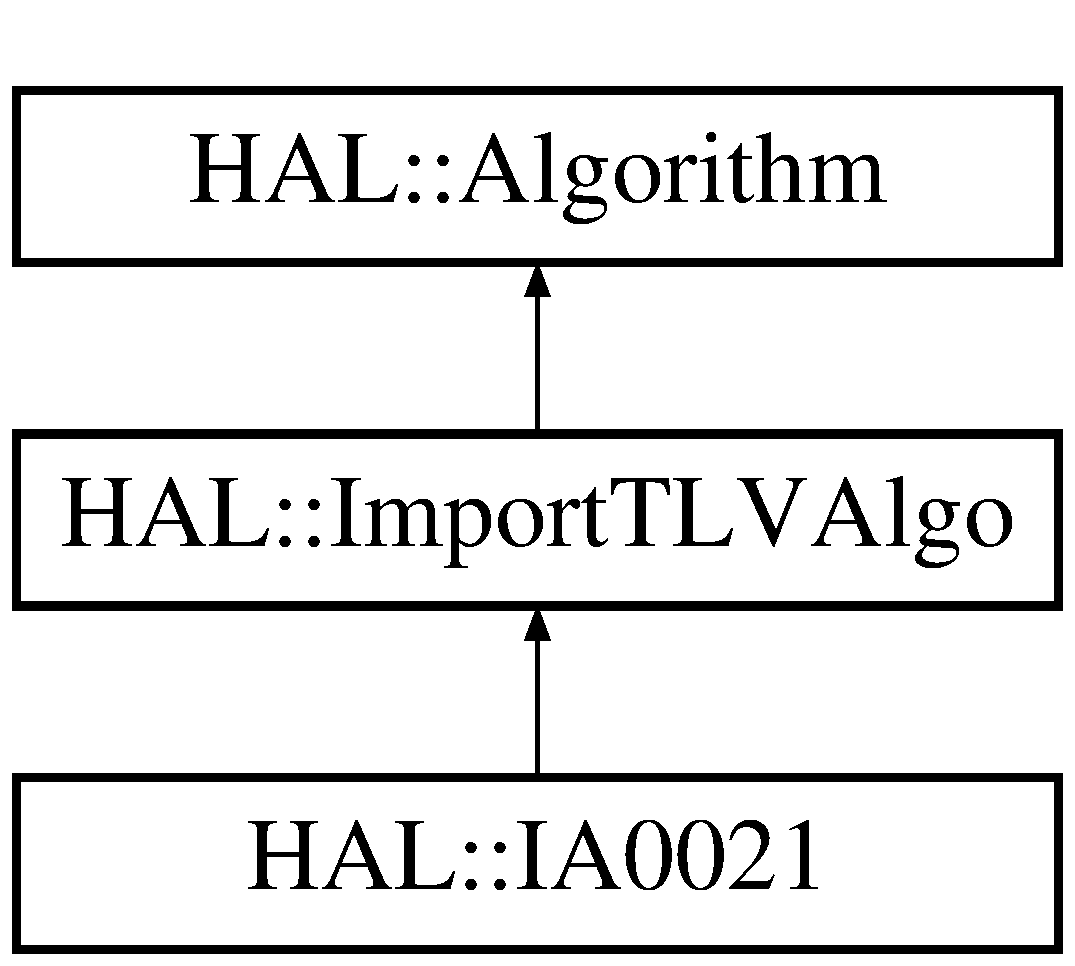
\includegraphics[height=3.000000cm]{class_h_a_l_1_1_i_a0021}
\end{center}
\end{figure}
\subsection*{Public Member Functions}
\begin{DoxyCompactItemize}
\item 
\hypertarget{class_h_a_l_1_1_i_a0021_aea44683ea1913cda29acdc00a8831c2d}{{\bfseries I\-A0021} (T\-String name, T\-String title)}\label{class_h_a_l_1_1_i_a0021_aea44683ea1913cda29acdc00a8831c2d}

\end{DoxyCompactItemize}
\subsection*{Protected Member Functions}
\begin{DoxyCompactItemize}
\item 
\hypertarget{class_h_a_l_1_1_i_a0021_ade49ac03e72a5ca25426efcc5c882e31}{virtual void {\bfseries Exec} (Option\-\_\-t $\ast$)}\label{class_h_a_l_1_1_i_a0021_ade49ac03e72a5ca25426efcc5c882e31}

\item 
\hypertarget{class_h_a_l_1_1_i_a0021_a80de69cebc7163a2ac15c0690f655b66}{virtual T\-Lorentz\-Vector $\ast$ {\bfseries Make\-T\-L\-V} (unsigned)}\label{class_h_a_l_1_1_i_a0021_a80de69cebc7163a2ac15c0690f655b66}

\end{DoxyCompactItemize}
\subsection*{Additional Inherited Members}


The documentation for this class was generated from the following file\-:\begin{DoxyCompactItemize}
\item 
/\-Users/jhetherly/src/root\-\_\-\-H\-A\-L/include/\-H\-A\-L/Algorithms.\-h\end{DoxyCompactItemize}

\hypertarget{class_h_a_l_1_1_i_a0022}{\section{H\-A\-L\-:\-:I\-A0022 Class Reference}
\label{class_h_a_l_1_1_i_a0022}\index{H\-A\-L\-::\-I\-A0022@{H\-A\-L\-::\-I\-A0022}}
}
Inheritance diagram for H\-A\-L\-:\-:I\-A0022\-:\begin{figure}[H]
\begin{center}
\leavevmode
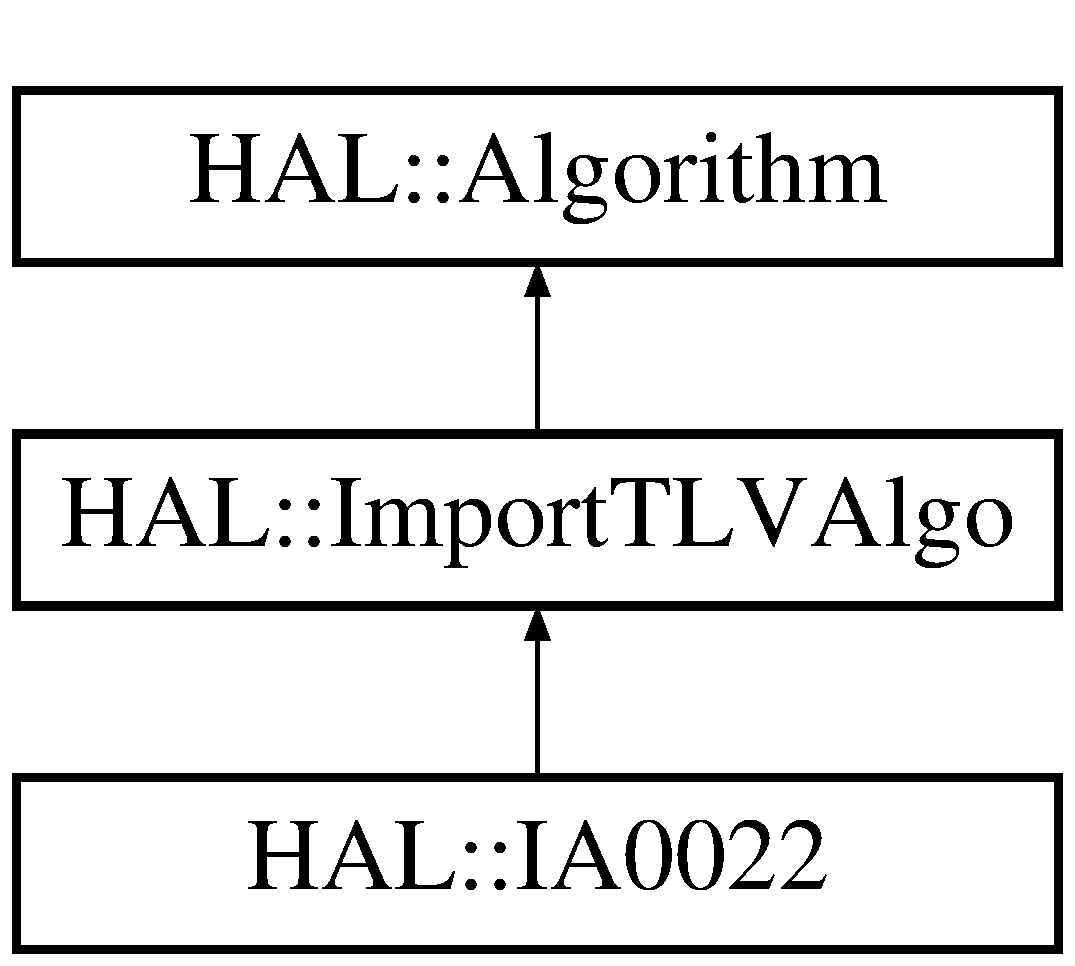
\includegraphics[height=3.000000cm]{class_h_a_l_1_1_i_a0022}
\end{center}
\end{figure}
\subsection*{Public Member Functions}
\begin{DoxyCompactItemize}
\item 
\hypertarget{class_h_a_l_1_1_i_a0022_a48f4c965f951daf7b2c385a9b130c83b}{{\bfseries I\-A0022} (T\-String name, T\-String title, unsigned n)}\label{class_h_a_l_1_1_i_a0022_a48f4c965f951daf7b2c385a9b130c83b}

\end{DoxyCompactItemize}
\subsection*{Protected Member Functions}
\begin{DoxyCompactItemize}
\item 
\hypertarget{class_h_a_l_1_1_i_a0022_a05dd9817ef69c14764f0df25376b8416}{virtual void {\bfseries Exec} (Option\-\_\-t $\ast$)}\label{class_h_a_l_1_1_i_a0022_a05dd9817ef69c14764f0df25376b8416}

\item 
\hypertarget{class_h_a_l_1_1_i_a0022_a919cc866aebae44cbf5dbcaeb09ace3d}{virtual T\-Lorentz\-Vector $\ast$ {\bfseries Make\-T\-L\-V} (unsigned)}\label{class_h_a_l_1_1_i_a0022_a919cc866aebae44cbf5dbcaeb09ace3d}

\end{DoxyCompactItemize}
\subsection*{Additional Inherited Members}


The documentation for this class was generated from the following file\-:\begin{DoxyCompactItemize}
\item 
/\-Users/jhetherly/src/root\-\_\-\-H\-A\-L/include/\-H\-A\-L/Algorithms.\-h\end{DoxyCompactItemize}

\hypertarget{class_h_a_l_1_1_import_t_l_v_algo}{\section{H\-A\-L\-:\-:Import\-T\-L\-V\-Algo Class Reference}
\label{class_h_a_l_1_1_import_t_l_v_algo}\index{H\-A\-L\-::\-Import\-T\-L\-V\-Algo@{H\-A\-L\-::\-Import\-T\-L\-V\-Algo}}
}
Inheritance diagram for H\-A\-L\-:\-:Import\-T\-L\-V\-Algo\-:\begin{figure}[H]
\begin{center}
\leavevmode
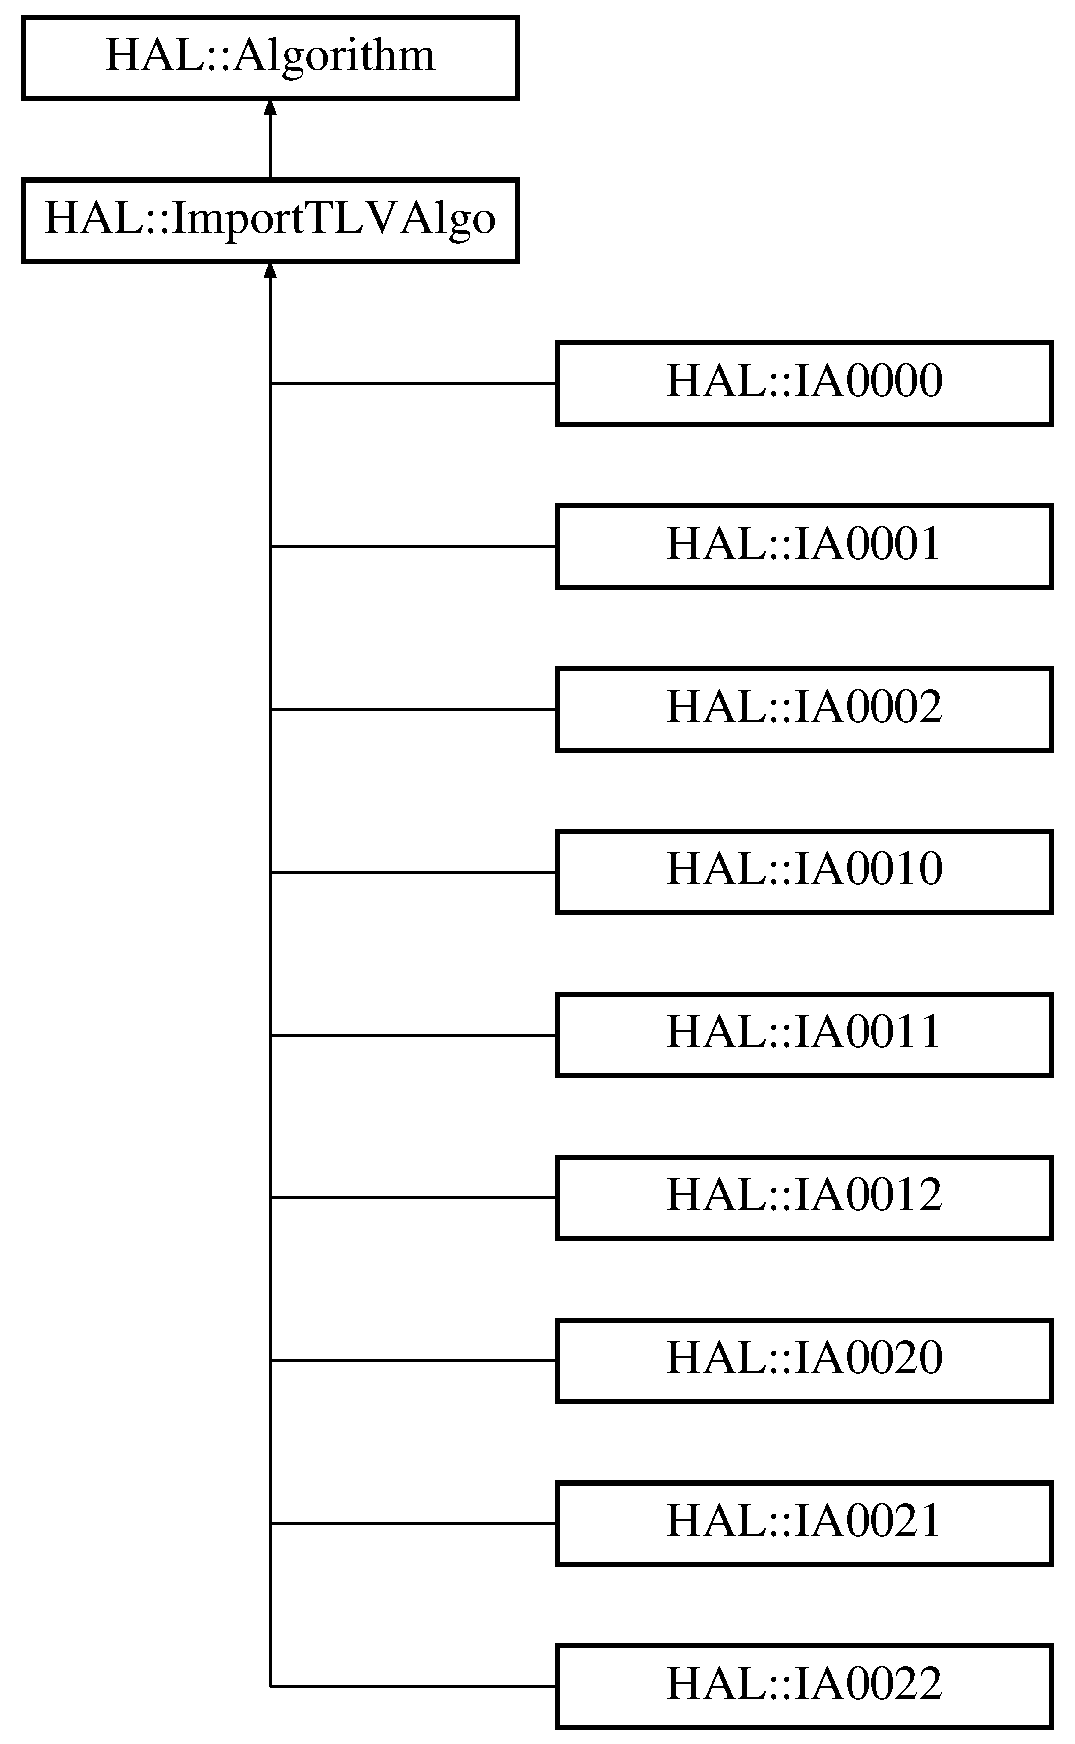
\includegraphics[height=11.000000cm]{class_h_a_l_1_1_import_t_l_v_algo}
\end{center}
\end{figure}
\subsection*{Public Member Functions}
\begin{DoxyCompactItemize}
\item 
\hypertarget{class_h_a_l_1_1_import_t_l_v_algo_a322b47d4ec39ca216268068b72e7446d}{{\bfseries Import\-T\-L\-V\-Algo} (T\-String name, T\-String title)}\label{class_h_a_l_1_1_import_t_l_v_algo_a322b47d4ec39ca216268068b72e7446d}

\end{DoxyCompactItemize}
\subsection*{Protected Member Functions}
\begin{DoxyCompactItemize}
\item 
\hypertarget{class_h_a_l_1_1_import_t_l_v_algo_aedad6d4046eea13e361b4104e44217ca}{virtual void {\bfseries Exec} (Option\-\_\-t $\ast$)}\label{class_h_a_l_1_1_import_t_l_v_algo_aedad6d4046eea13e361b4104e44217ca}

\item 
\hypertarget{class_h_a_l_1_1_import_t_l_v_algo_a244c49b3d20537f089452c911dc18dfc}{virtual void {\bfseries Exec} (unsigned n)}\label{class_h_a_l_1_1_import_t_l_v_algo_a244c49b3d20537f089452c911dc18dfc}

\item 
\hypertarget{class_h_a_l_1_1_import_t_l_v_algo_aa9af7bb8a480bb31434f4e1c53cddd66}{virtual void {\bfseries Clear} (Option\-\_\-t $\ast$)}\label{class_h_a_l_1_1_import_t_l_v_algo_aa9af7bb8a480bb31434f4e1c53cddd66}

\item 
\hypertarget{class_h_a_l_1_1_import_t_l_v_algo_a46386035cffeea3764f49ca0fb3280e3}{virtual T\-Lorentz\-Vector $\ast$ {\bfseries Make\-T\-L\-V} (unsigned)=0}\label{class_h_a_l_1_1_import_t_l_v_algo_a46386035cffeea3764f49ca0fb3280e3}

\end{DoxyCompactItemize}
\subsection*{Additional Inherited Members}


The documentation for this class was generated from the following file\-:\begin{DoxyCompactItemize}
\item 
/\-Users/jhetherly/src/root\-\_\-\-H\-A\-L/include/\-H\-A\-L/Algorithms.\-h\end{DoxyCompactItemize}

\hypertarget{class_h_a_l_1_1_integrator}{\section{H\+A\+L\+:\+:Integrator Class Reference}
\label{class_h_a_l_1_1_integrator}\index{H\+A\+L\+::\+Integrator@{H\+A\+L\+::\+Integrator}}
}
\subsection*{Public Member Functions}
\begin{DoxyCompactItemize}
\item 
\hypertarget{class_h_a_l_1_1_integrator_acd878eaa888dfce44a3c1130770a74a5}{{\bfseries Integrator} (const Double\+\_\+t \&tolerance=1.\+0e-\/12)}\label{class_h_a_l_1_1_integrator_acd878eaa888dfce44a3c1130770a74a5}

\item 
\hypertarget{class_h_a_l_1_1_integrator_a5eefbd36726dbcaaabb07cd617799661}{{\footnotesize template$<$class T $>$ }\\Double\+\_\+t {\bfseries Integrate} (T \&, const Double\+\_\+t \&lower\+\_\+bound, const Double\+\_\+t \&upper\+\_\+bound)}\label{class_h_a_l_1_1_integrator_a5eefbd36726dbcaaabb07cd617799661}

\item 
\hypertarget{class_h_a_l_1_1_integrator_ab866da7ce3499bcf3d874fac6ef1e6fc}{Bool\+\_\+t {\bfseries Out\+Of\+Tolerance} ()}\label{class_h_a_l_1_1_integrator_ab866da7ce3499bcf3d874fac6ef1e6fc}

\end{DoxyCompactItemize}


The documentation for this class was generated from the following file\+:\begin{DoxyCompactItemize}
\item 
/\+Users/jhetherly/src/root\+\_\+\+H\+A\+L/include/\+H\+A\+L/Integrator.\+h\end{DoxyCompactItemize}

\hypertarget{class_h_a_l_1_1_interp_base}{\section{H\+A\+L\+:\+:Interp\+Base Class Reference}
\label{class_h_a_l_1_1_interp_base}\index{H\+A\+L\+::\+Interp\+Base@{H\+A\+L\+::\+Interp\+Base}}
}
Inheritance diagram for H\+A\+L\+:\+:Interp\+Base\+:\begin{figure}[H]
\begin{center}
\leavevmode
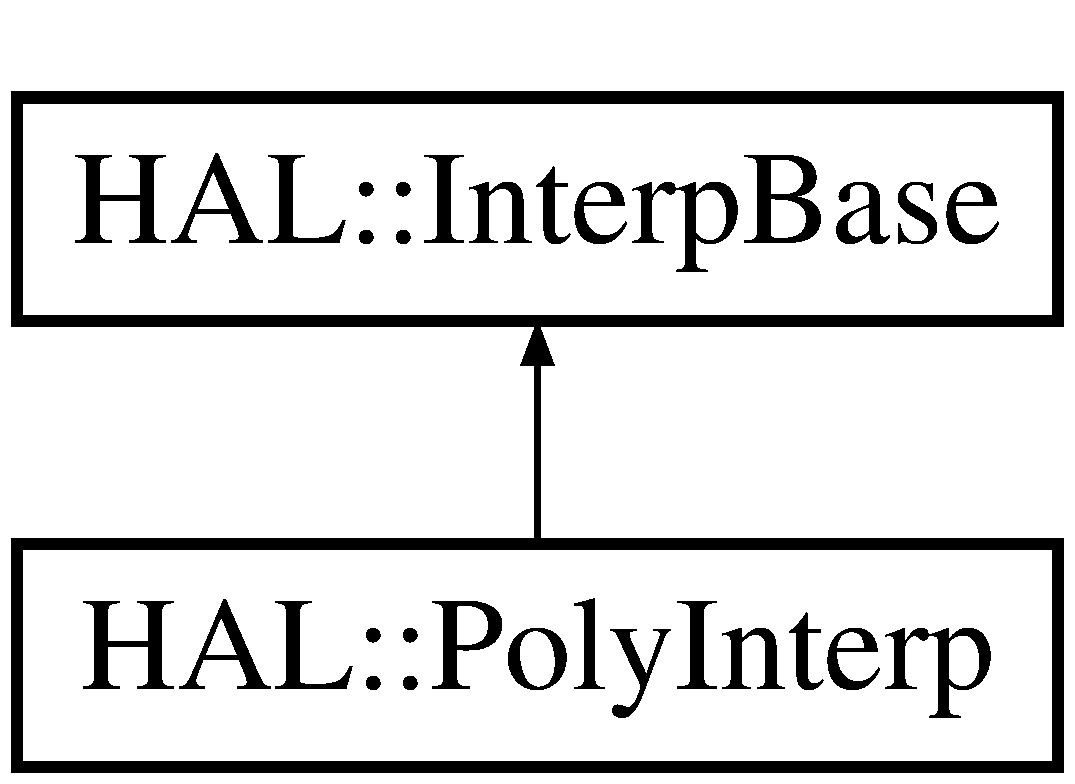
\includegraphics[height=2.000000cm]{class_h_a_l_1_1_interp_base}
\end{center}
\end{figure}
\subsection*{Public Member Functions}
\begin{DoxyCompactItemize}
\item 
\hypertarget{class_h_a_l_1_1_interp_base_a7da5f00617f93f337e983e48faa339d7}{{\bfseries Interp\+Base} (Double\+\_\+t $\ast$x, Double\+\_\+t $\ast$y, Int\+\_\+t xs, Int\+\_\+t m)}\label{class_h_a_l_1_1_interp_base_a7da5f00617f93f337e983e48faa339d7}

\item 
\hypertarget{class_h_a_l_1_1_interp_base_a54d32cf70679d2eb8d1a39a0bd242b39}{Int\+\_\+t {\bfseries locate} (const Double\+\_\+t \&x)}\label{class_h_a_l_1_1_interp_base_a54d32cf70679d2eb8d1a39a0bd242b39}

\item 
\hypertarget{class_h_a_l_1_1_interp_base_ad1bccffef0b532774150b419dbdff5b3}{Int\+\_\+t {\bfseries hunt} (const Double\+\_\+t \&x)}\label{class_h_a_l_1_1_interp_base_ad1bccffef0b532774150b419dbdff5b3}

\item 
\hypertarget{class_h_a_l_1_1_interp_base_a7d86cc16a9c8ba0bf24e8137f9eb21b3}{Double\+\_\+t {\bfseries Interp} (const Double\+\_\+t \&x)}\label{class_h_a_l_1_1_interp_base_a7d86cc16a9c8ba0bf24e8137f9eb21b3}

\item 
\hypertarget{class_h_a_l_1_1_interp_base_a524cc9b36f0e36c8f69f5c77bc68de7b}{virtual Double\+\_\+t {\bfseries rawinterp} (const Int\+\_\+t \&jlo, const Double\+\_\+t \&x)=0}\label{class_h_a_l_1_1_interp_base_a524cc9b36f0e36c8f69f5c77bc68de7b}

\end{DoxyCompactItemize}
\subsection*{Public Attributes}
\begin{DoxyCompactItemize}
\item 
\hypertarget{class_h_a_l_1_1_interp_base_a70c78b7c0ba2fe8a5ac3091ebb70f1ae}{Int\+\_\+t {\bfseries n}}\label{class_h_a_l_1_1_interp_base_a70c78b7c0ba2fe8a5ac3091ebb70f1ae}

\item 
\hypertarget{class_h_a_l_1_1_interp_base_a8691b520d0856373d8763be3cf0a9082}{Int\+\_\+t {\bfseries mm}}\label{class_h_a_l_1_1_interp_base_a8691b520d0856373d8763be3cf0a9082}

\item 
\hypertarget{class_h_a_l_1_1_interp_base_acfe70f15b2295e6b2399c02802072c9c}{Int\+\_\+t {\bfseries cor}}\label{class_h_a_l_1_1_interp_base_acfe70f15b2295e6b2399c02802072c9c}

\item 
\hypertarget{class_h_a_l_1_1_interp_base_a76921f15cd1908cdbe5bcc6afeb1ecc4}{Int\+\_\+t {\bfseries jsav}}\label{class_h_a_l_1_1_interp_base_a76921f15cd1908cdbe5bcc6afeb1ecc4}

\item 
\hypertarget{class_h_a_l_1_1_interp_base_af433768e4c59a1209919246ecb991c86}{Int\+\_\+t {\bfseries dj}}\label{class_h_a_l_1_1_interp_base_af433768e4c59a1209919246ecb991c86}

\item 
\hypertarget{class_h_a_l_1_1_interp_base_acdfb5ae98e96886c9055f36d29ebd25e}{Double\+\_\+t $\ast$ {\bfseries xx}}\label{class_h_a_l_1_1_interp_base_acdfb5ae98e96886c9055f36d29ebd25e}

\item 
\hypertarget{class_h_a_l_1_1_interp_base_a49d9cd794e1c97a0ed3f3bab3a999b8b}{Double\+\_\+t $\ast$ {\bfseries yy}}\label{class_h_a_l_1_1_interp_base_a49d9cd794e1c97a0ed3f3bab3a999b8b}

\end{DoxyCompactItemize}


The documentation for this class was generated from the following file\+:\begin{DoxyCompactItemize}
\item 
/\+Users/jhetherly/src/\+H\+A\+L-\/\+R\+O\+O\+T/include/\+H\+A\+L/Interpolator.\+h\end{DoxyCompactItemize}

\hypertarget{class_h_a_l_1_1_poly2_d_interp}{\section{H\+A\+L\+:\+:Poly2\+D\+Interp Class Reference}
\label{class_h_a_l_1_1_poly2_d_interp}\index{H\+A\+L\+::\+Poly2\+D\+Interp@{H\+A\+L\+::\+Poly2\+D\+Interp}}
}
\subsection*{Public Member Functions}
\begin{DoxyCompactItemize}
\item 
\hypertarget{class_h_a_l_1_1_poly2_d_interp_a2e06fafe80eb98739813a67a1f5b5f89}{{\bfseries Poly2\+D\+Interp} (Double\+\_\+t $\ast$x1\+\_\+values, Double\+\_\+t $\ast$x2\+\_\+values, Int\+\_\+t x1\+\_\+size, Int\+\_\+t x2\+\_\+size, Double\+\_\+t $\ast$$\ast$y\+\_\+matrix, Int\+\_\+t x1\+\_\+order, Int\+\_\+t x2\+\_\+order)}\label{class_h_a_l_1_1_poly2_d_interp_a2e06fafe80eb98739813a67a1f5b5f89}

\item 
\hypertarget{class_h_a_l_1_1_poly2_d_interp_aaeda2c3c4e09d48611973dcd95940756}{Double\+\_\+t {\bfseries Interp} (const Double\+\_\+t \&x1\+\_\+value, const Double\+\_\+t \&x2\+\_\+value)}\label{class_h_a_l_1_1_poly2_d_interp_aaeda2c3c4e09d48611973dcd95940756}

\item 
\hypertarget{class_h_a_l_1_1_poly2_d_interp_a3488ef8691d670a5f2170a9ebead44d7}{Double\+\_\+t {\bfseries Get\+X1\+Error} ()}\label{class_h_a_l_1_1_poly2_d_interp_a3488ef8691d670a5f2170a9ebead44d7}

\item 
\hypertarget{class_h_a_l_1_1_poly2_d_interp_a9d7ab5e66ee29fe41187d39086152dfe}{Double\+\_\+t {\bfseries Get\+X2\+Error} ()}\label{class_h_a_l_1_1_poly2_d_interp_a9d7ab5e66ee29fe41187d39086152dfe}

\end{DoxyCompactItemize}
\subsection*{Public Attributes}
\begin{DoxyCompactItemize}
\item 
\hypertarget{class_h_a_l_1_1_poly2_d_interp_af07844f91abbfa62348292ae16a90fdc}{Double\+\_\+t $\ast$$\ast$ {\bfseries y}}\label{class_h_a_l_1_1_poly2_d_interp_af07844f91abbfa62348292ae16a90fdc}

\end{DoxyCompactItemize}


The documentation for this class was generated from the following file\+:\begin{DoxyCompactItemize}
\item 
/\+Users/jhetherly/src/root\+\_\+\+H\+A\+L/include/\+H\+A\+L/Interpolator.\+h\end{DoxyCompactItemize}

\hypertarget{class_h_a_l_1_1_poly_interp}{\section{H\+A\+L\+:\+:Poly\+Interp Class Reference}
\label{class_h_a_l_1_1_poly_interp}\index{H\+A\+L\+::\+Poly\+Interp@{H\+A\+L\+::\+Poly\+Interp}}
}
Inheritance diagram for H\+A\+L\+:\+:Poly\+Interp\+:\begin{figure}[H]
\begin{center}
\leavevmode
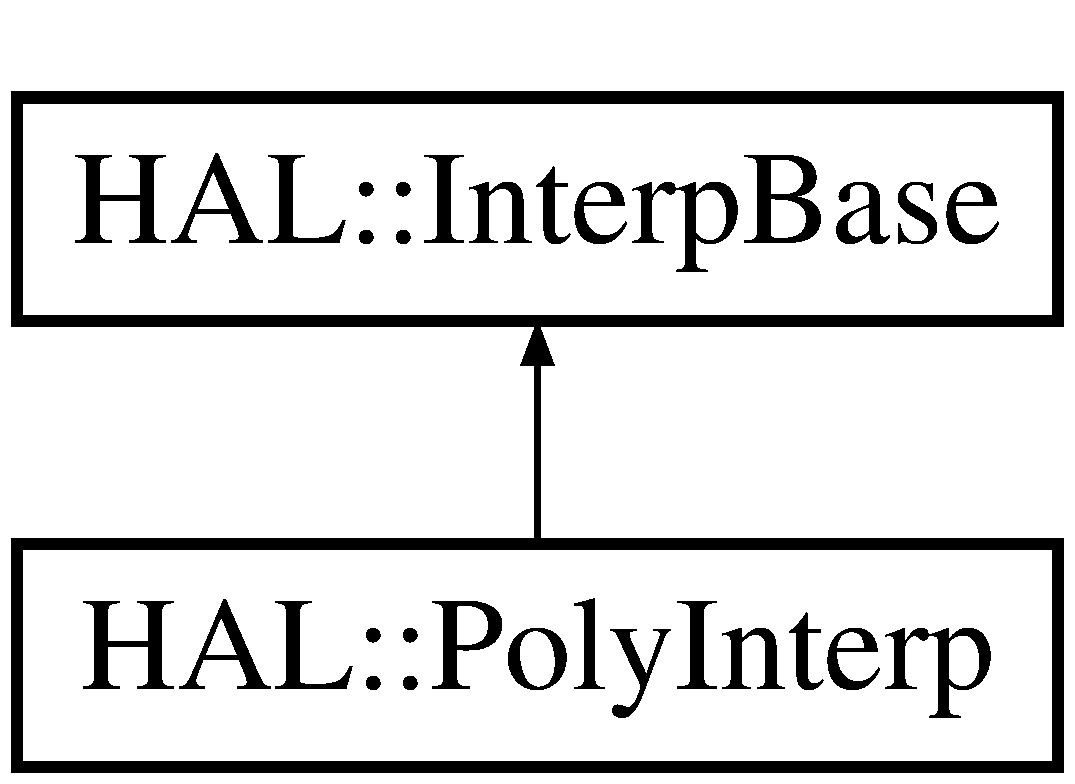
\includegraphics[height=2.000000cm]{class_h_a_l_1_1_poly_interp}
\end{center}
\end{figure}
\subsection*{Public Member Functions}
\begin{DoxyCompactItemize}
\item 
\hypertarget{class_h_a_l_1_1_poly_interp_af44f92e27052c066755a5beae2dc7b1b}{{\bfseries Poly\+Interp} (Double\+\_\+t $\ast$x\+\_\+values, Double\+\_\+t $\ast$y\+\_\+values, Int\+\_\+t size, Int\+\_\+t order)}\label{class_h_a_l_1_1_poly_interp_af44f92e27052c066755a5beae2dc7b1b}

\item 
\hypertarget{class_h_a_l_1_1_poly_interp_a1d87892f07ecdacaf6467a63371f044e}{Double\+\_\+t {\bfseries Get\+Error} ()}\label{class_h_a_l_1_1_poly_interp_a1d87892f07ecdacaf6467a63371f044e}

\end{DoxyCompactItemize}
\subsection*{Friends}
\begin{DoxyCompactItemize}
\item 
\hypertarget{class_h_a_l_1_1_poly_interp_a1d517ab352221a0d0a7fbfc8698724d7}{class {\bfseries Poly2\+D\+Interp}}\label{class_h_a_l_1_1_poly_interp_a1d517ab352221a0d0a7fbfc8698724d7}

\end{DoxyCompactItemize}
\subsection*{Additional Inherited Members}


The documentation for this class was generated from the following file\+:\begin{DoxyCompactItemize}
\item 
/\+Users/jhetherly/src/\+H\+A\+L-\/\+R\+O\+O\+T/include/\+H\+A\+L/Interpolator.\+h\end{DoxyCompactItemize}

\hypertarget{class_h_a_l_1_1_python_reconstruction_algorithm}{\section{H\-A\-L\-:\-:Python\-Reconstruction\-Algorithm Class Reference}
\label{class_h_a_l_1_1_python_reconstruction_algorithm}\index{H\-A\-L\-::\-Python\-Reconstruction\-Algorithm@{H\-A\-L\-::\-Python\-Reconstruction\-Algorithm}}
}
Inheritance diagram for H\-A\-L\-:\-:Python\-Reconstruction\-Algorithm\-:\begin{figure}[H]
\begin{center}
\leavevmode
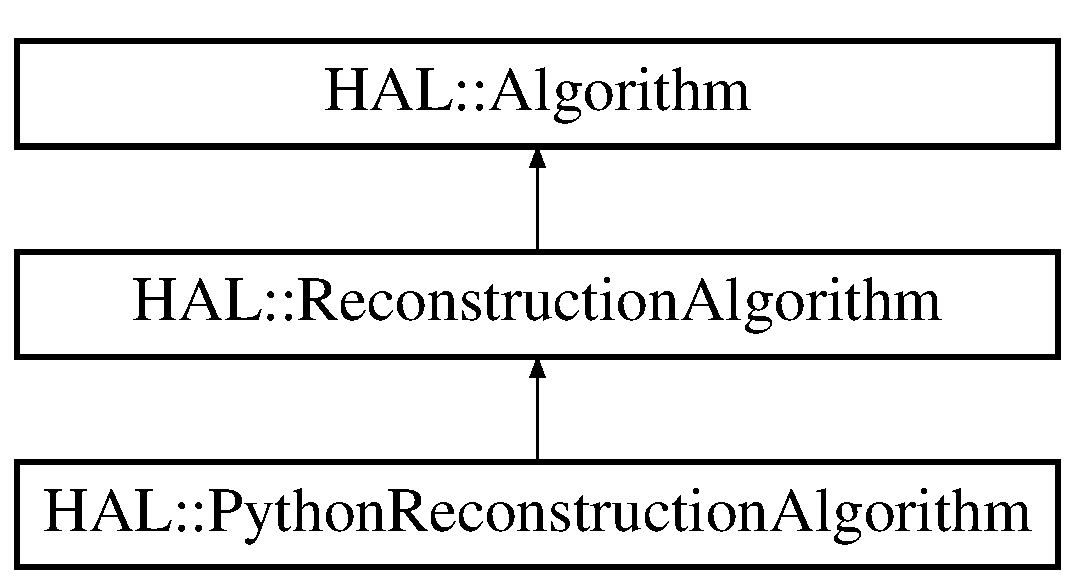
\includegraphics[height=3.000000cm]{class_h_a_l_1_1_python_reconstruction_algorithm}
\end{center}
\end{figure}
\subsection*{Public Member Functions}
\begin{DoxyCompactItemize}
\item 
\hypertarget{class_h_a_l_1_1_python_reconstruction_algorithm_a62fdc4403273df30ecd4cff5b09f5252}{{\bfseries Python\-Reconstruction\-Algorithm} (T\-String name=\char`\"{}\char`\"{}, T\-String title=\char`\"{}\char`\"{}, T\-String Py\-Path=\char`\"{}\char`\"{}, T\-String Py\-File=\char`\"{}\char`\"{}, T\-String Py\-Class=\char`\"{}\char`\"{}, Py\-Object $\ast$self=0)}\label{class_h_a_l_1_1_python_reconstruction_algorithm_a62fdc4403273df30ecd4cff5b09f5252}

\item 
\hypertarget{class_h_a_l_1_1_python_reconstruction_algorithm_aac27f846671212cdf0ca1e5dabb74f76}{virtual void {\bfseries Init} (Option\-\_\-t $\ast$options=\char`\"{}\char`\"{})}\label{class_h_a_l_1_1_python_reconstruction_algorithm_aac27f846671212cdf0ca1e5dabb74f76}

\item 
\hypertarget{class_h_a_l_1_1_python_reconstruction_algorithm_aebfd89f3b0fd586ad2bb224d5d84aa8f}{virtual void {\bfseries Exec} (Option\-\_\-t $\ast$options=\char`\"{}\char`\"{})}\label{class_h_a_l_1_1_python_reconstruction_algorithm_aebfd89f3b0fd586ad2bb224d5d84aa8f}

\item 
\hypertarget{class_h_a_l_1_1_python_reconstruction_algorithm_ab80718c499dcc01a8cca9f8894d92f87}{virtual void {\bfseries Clear} (Option\-\_\-t $\ast$options=\char`\"{}\char`\"{})}\label{class_h_a_l_1_1_python_reconstruction_algorithm_ab80718c499dcc01a8cca9f8894d92f87}

\end{DoxyCompactItemize}
\subsection*{Additional Inherited Members}


The documentation for this class was generated from the following file\-:\begin{DoxyCompactItemize}
\item 
/\-Users/jhetherly/src/root\-\_\-\-H\-A\-L/include/\-H\-A\-L/Python\-Reconstruction\-Algorithm.\-h\end{DoxyCompactItemize}

\hypertarget{class_h_a_l_1_1_reconstruction_algorithm}{\section{H\-A\-L\-:\-:Reconstruction\-Algorithm Class Reference}
\label{class_h_a_l_1_1_reconstruction_algorithm}\index{H\-A\-L\-::\-Reconstruction\-Algorithm@{H\-A\-L\-::\-Reconstruction\-Algorithm}}
}
Inheritance diagram for H\-A\-L\-:\-:Reconstruction\-Algorithm\-:\begin{figure}[H]
\begin{center}
\leavevmode
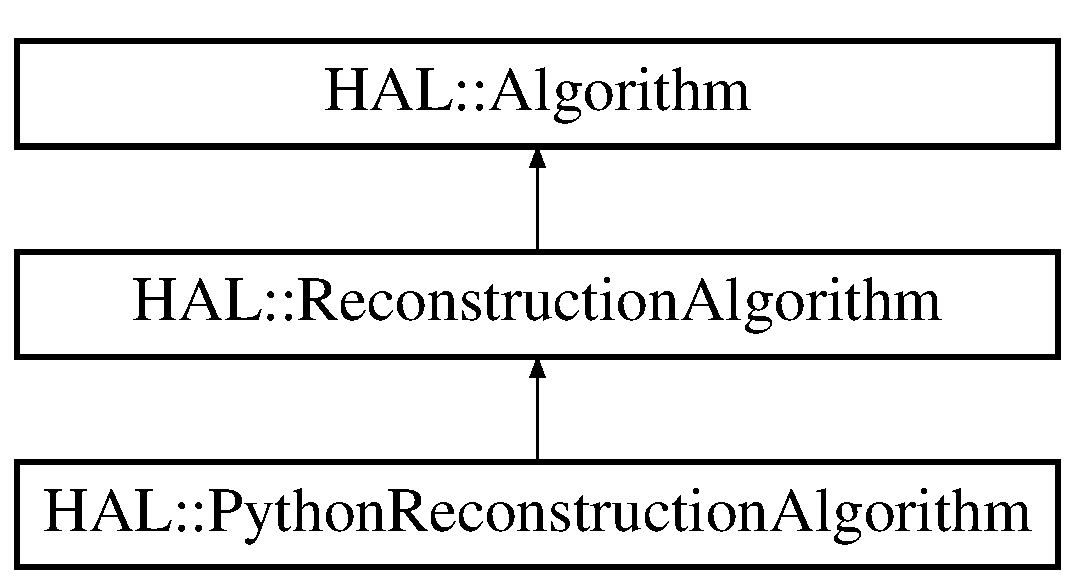
\includegraphics[height=3.000000cm]{class_h_a_l_1_1_reconstruction_algorithm}
\end{center}
\end{figure}
\subsection*{Public Member Functions}
\begin{DoxyCompactItemize}
\item 
\hypertarget{class_h_a_l_1_1_reconstruction_algorithm_ab384574a47016e7b1a93097d15782672}{{\bfseries Reconstruction\-Algorithm} (T\-String name=\char`\"{}\char`\"{}, T\-String title=\char`\"{}\char`\"{})}\label{class_h_a_l_1_1_reconstruction_algorithm_ab384574a47016e7b1a93097d15782672}

\end{DoxyCompactItemize}
\subsection*{Additional Inherited Members}


The documentation for this class was generated from the following file\-:\begin{DoxyCompactItemize}
\item 
/\-Users/jhetherly/src/root\-\_\-\-H\-A\-L/include/\-H\-A\-L/Reconstruction\-Algorithm.\-h\end{DoxyCompactItemize}

\addcontentsline{toc}{part}{Index}
\printindex
\end{document}
